%%%%%%%%%%%%%%%%%%%%%%%%%%%%%%%%%%%%%%%%%
% Thin Sectioned Essay
% LaTeX Template
% Version 1.0 (3/8/13)
%
% This template has been downloaded from:
% http://www.LaTeXTemplates.com
%
% Original Author:
% Nicolas Diaz (nsdiaz@uc.cl) with extensive modifications by:
% Vel (vel@latextemplates.com)
%
% License:
% CC BY-NC-SA 3.0 (http://creativecommons.org/licenses/by-nc-sa/3.0/)
%
%%%%%%%%%%%%%%%%%%%%%%%%%%%%%%%%%%%%%%%%%

%----------------------------------------------------------------------------------------
%	PACKAGES AND OTHER DOCUMENT CONFIGURATIONS
%----------------------------------------------------------------------------------------

\documentclass[a3paper, 12pt]{book} % Font size (can be 10pt, 11pt or 12pt) and paper size (remove a4paper for US letter paper)

\usepackage[protrusion=true,expansion=true]{microtype} % Better typography
\usepackage{graphicx} % Required for including pictures
\usepackage{wrapfig} % Allows in-line images

\usepackage{algorithmic}
\usepackage{CJKutf8}
\usepackage{listings}
\usepackage{color}
\usepackage{centernot}
\usepackage{bm}
\usepackage{natbib}
\usepackage{amssymb}
\usepackage{hyperref}

\newcommand\bolden[1]{{\boldmath\bfseries#1}}
\definecolor{dkgreen}{rgb}{0,0.6,0}
\definecolor{mauve}{rgb}{0.58,0,0.82}

\lstset{frame=tb,
	language=Python,
	aboveskip=3mm,
	belowskip=3mm,
	showstringspaces=false,
	columns=flexible,
	basicstyle={\small\ttfamily},
	numbers=none,
	numberstyle=\tiny\color{gray},
	keywordstyle=\color{blue},
	commentstyle=\color{dkgreen},
	stringstyle=\color{mauve},
	breaklines=true,
	breakatwhitespace=true,
	tabsize=3
}


\usepackage{enumitem}
\usepackage{amsmath}
\usepackage{mathpazo} % Use the Palatino font
\usepackage[T1]{fontenc} % Required for accented characters
\linespread{1.05} % Change line spacing here, Palatino benefits from a slight increase by default

\newcommand{\CI}{\mathrel{\perp\mspace{-10mu}\perp}}
\newcommand{\nCI}{\centernot{\CI}}

\makeatletter
\renewcommand\@biblabel[1]{\textbf{#1.}} % Change the square brackets for each bibliography item from '[1]' to '1.'
\renewcommand{\@listI}{\itemsep=0pt} % Reduce the space between items in the itemize and enumerate environments and the bibliography

\renewcommand{\maketitle}{ % Customize the title - do not edit title and author name here, see the TITLE block below
\begin{flushright} % Right align
{\LARGE\@title} % Increase the font size of the title

\vspace{50pt} % Some vertical space between the title and author name

{\large\@author} % Author name
\\\@date % Date

\vspace{40pt} % Some vertical space between the author block and abstract
\end{flushright}
}

%----------------------------------------------------------------------------------------
%	TITLE
%----------------------------------------------------------------------------------------

\title{\textbf{Learning Notes on Computer Science and Artificial Intelligence}\\ % Title
} % Subtitle

\author{\textsc{Jian Tong} % Author
\\{\textit{University of Edinburgh}}} % Institution

\date{\today} % Date

%----------------------------------------------------------------------------------------

\begin{document}

\maketitle % Print the title section

\vspace{30pt} % Some vertical space between the abstract and first section

%----------------------------------------------------------------------------------------
%	ESSAY BODY
%----------------------------------------------------------------------------------------
\part{Natural Language Processing}

%------------------------------------------------

\chapter{Vector Semantics}
\section{Skip-gram}
\citep{mikolov2013distributed} proposed Skip-gram model whose training objective is to find word representations useful for predicting the \textbf{surrounding words} in a sentence or a document. Given a sequence of training words $w_1,w_2,w_3,...,w_T$, the objective is to maximize the average log probability

$$\frac{1}{T}\sum_{t=1}^{T}{\sum_{-c\le{j\le{c}}}{\log(w_{t+j}|w_t)}}$$
The basic Skip-gram formulation defines $p(w_{t+j}|w_t)$ using softmax function:

$$p(w_O|w_I)=\frac{\exp{(\bar{v}_{w_{O}}^{\top}v_{w_{I}})}}{\sum_{w=1}^{W}{\exp{(\bar{v}_{w}^{\top}v_{w_{I}})}}}$$ \\

\begin{figure}[htpb]
	\centering
	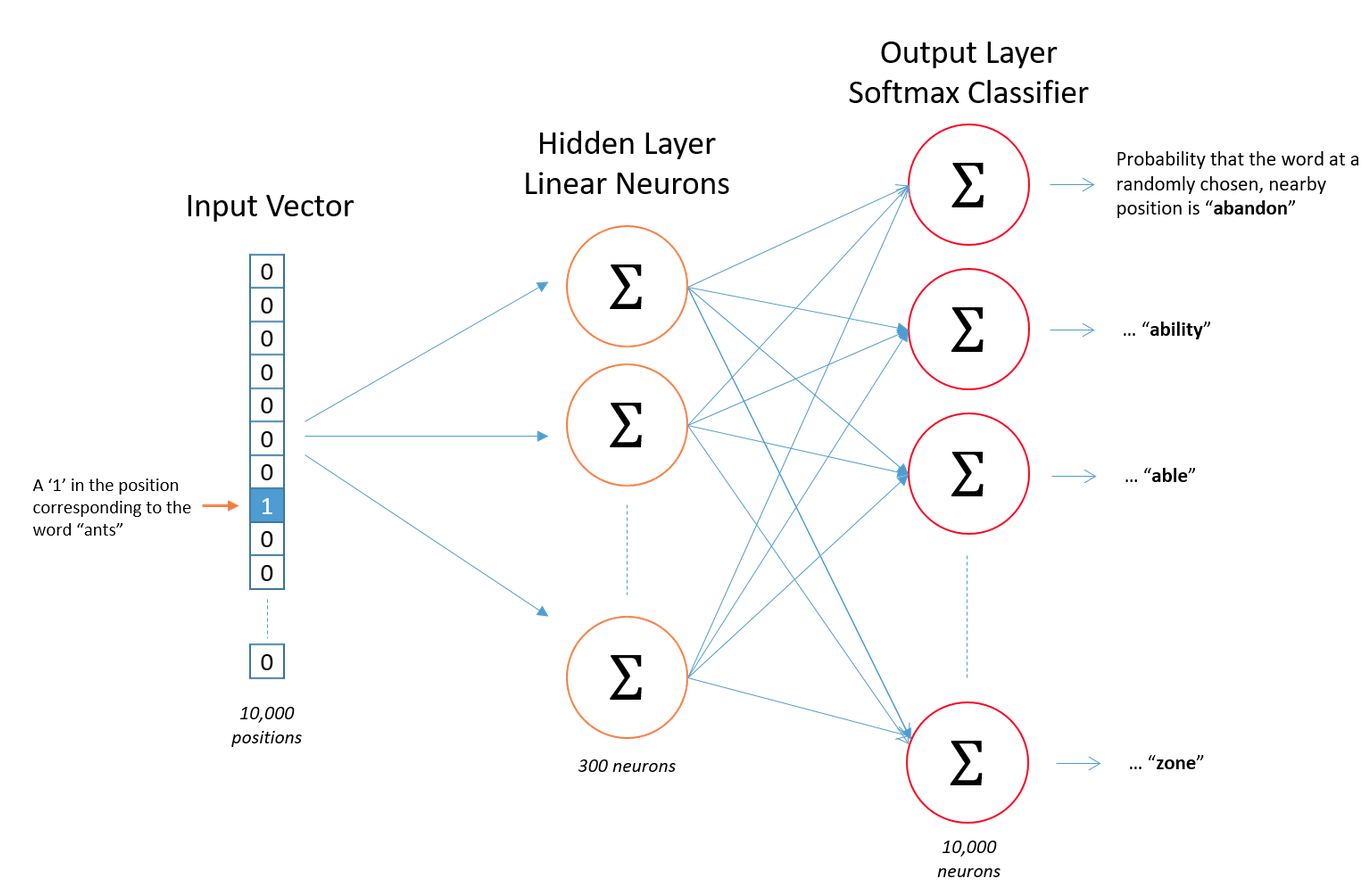
\includegraphics[width=8cm]{figures/skip_gram_architecture.png}
	\caption{Neural network architecture of Skip-gram model}
	\label{fig:skip_gram}
\end{figure}

The architecture of Skip-gram model is shown in Figure \ref{fig:skip_gram}, it should be noticed that the model is a \textbf{two-layer} network(hidden units and output units),which leads to one of its drawbacks --- $p(w_{j+t}|w_t)$ is \textbf{asymmetric}, that is, $p(w_2|w_1)$ is not necessarily equal to $p(w_1|w_2)$. We need to separate the vector space between target words and context words. (\textbf{hidden units} and \textbf{output units})


\section{GloVe}
\textbf{GloVe} or \textbf{Global Vector} \citep{pennington2014glove}, directly captures the global corpus statistics. The model attempts to solve two respective problems in word vector learning algorithms:

\begin{itemize}
	\item \textbf{global matrix factorization}: do relatively poorly on the word analogy task, indicating a sub-optimal vector space structure. 
	\item \textbf{local context window}: poorly utilize the statistics of the corpus since they train on separate local context windows instead of on global co-occurrence counts.
\end{itemize}

Let word-word co-occurrence counts be denoted by $X_{ij}$, denotes the number of times word $j$ occurs in the context of word $i$. The \textbf{ratios of co-occurrence probabilities} rather than the \textbf{probabilities} themselves provide useful information.

\begin{figure}[htpb]
	\centering
	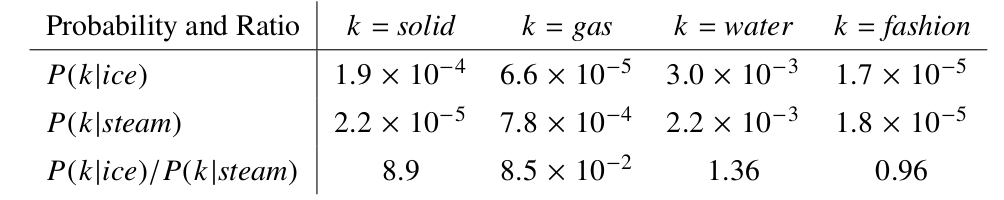
\includegraphics[width=9.5cm]{figures/glove_co-occurrence_ratio.png}
	\caption{ratio of co-occurrence probabilities}
	\label{fig:glove_co-occurrence_ratio}
\end{figure}

As shown in Figure \ref{fig:glove_co-occurrence_ratio} , only the ratios noise from non-discriminative  words like \emph{water} and \emph{fashion} cancel out, so the large values (much greater than $1$) correlate well with properties specific to ice, and small values (much less than $1$) correlate well with specific properties of steam.

\subsection{Model Interpretation}

The most general model takes the form, where $w \in \mathbb{R}^{d}$ are \textbf{word vectors} and $\tilde{w} \in \mathbb{R}^{d}$ are \textbf{separate context vectors}. Let $P_{ij}=P(j|i)=X_{i,j}/X_i$ be the probability that \textbf{word $j$ appear in the context of word $i$}.
$$F(w_i, w_j, \tilde{w}_k) = \frac{P_{ik}}{P_{jk}}$$
Since vector spaces are inherently linear structures, the most natural way to do this is vector differences
$$F(w_i-w_j, \tilde{w}_k) = \frac{P_{ik}}{P_{jk}}$$
In order to make the left-hand side as a scalar
$$F((w_i-w_j)^{\top}\tilde{w}_k) = \frac{P_{ik}}{P_{jk}}$$
To remove the distinction between context vectors and word vectors, symmetry need to be restored. $F$ is required to be homomorphism between the groups ($\mathbb{R}$, +) and ($\mathbb{R}$, $\times$), i.e.,
$$F((w_i-w_j)^{\top}\tilde{w}_k) = \frac{F(w_i^{\top}\tilde{w}_k)}{F(w_j^{\top}\tilde{w}_k)}$$
$$F(w_i^{\top}\tilde{w}_k) = P_{ik} = \frac{X_{ik}}{X_i}$$
The solution is $F=\exp$, or, 
$$ w_i^{\top}\tilde{w}_k = \log{(P_{ik})} = \log{(X_{ik})}-\log{(X_{i})}$$
Noted that it would exhibit the exchange symmetry if not for the $\log{(X_i)}$ on the right-hand side. However, this term is independent of $k$ so it can be absorbed into a bias $b_i$ for $w_i$. Finally, adding an additional bias $\tilde{b}_k$ for  $\tilde{w}_k$ restores the symmetry
$$ w_i^{\top}\tilde{w}_k +  b_i + \tilde{b}_k = \log{(X_{ik})}$$

Two tricks are introduced here as follows:
\begin{itemize}
	\item \textbf{logarithm divergence}
	\item \textbf{weigh all co-occurrences equally}
\end{itemize}
One resolution is to include an additive shift in the logarithm, $\log{(X_{ik})} \to \log{(1+X_{ik})}$, which maintains the sparsity of $X$ while avoiding divergence. But GloVe introduces a new weighting function $f(X_{ij})$ into the cost function to solve these two problems simultaneously
$$J=\sum_{i,j=1}^{V}{f(X_{ij})(w_i^{\top}\tilde{w}_k +  b_i + \tilde{b}_k - \log{X_{ij}})^2}$$

$f(x)=(x/x_{max})^\alpha$ if $x \le x_{max}$ \\
\indent $f(x)=1$ otherwise \\

which has the following properties
\begin{enumerate}
	\item $f(0)=0$.
	\item $f(x)$ should be non-decreasing so that rare co-occurrences are not overweighted.
	\item $f(x)$ should be relatively small for large values of $x$, so that frequent co-occurrences are
	not overweighted.
\end{enumerate}

\subsection{Time Complexity}

we conclude that the complexity of the model is much better than the \textbf{worst case} $O(V^2)$,and in fact it does somewhat better than the on-line window-based methods which scale like $O(|C|)$.

\section{FastText}
In many \textbf{morphologically rich} languages like Finnish, French and Spanish, \citep{bojanowski2016enriching} it is possible to improve vector representations by using character level information.

\begin{figure}[htpb]
	\centering
	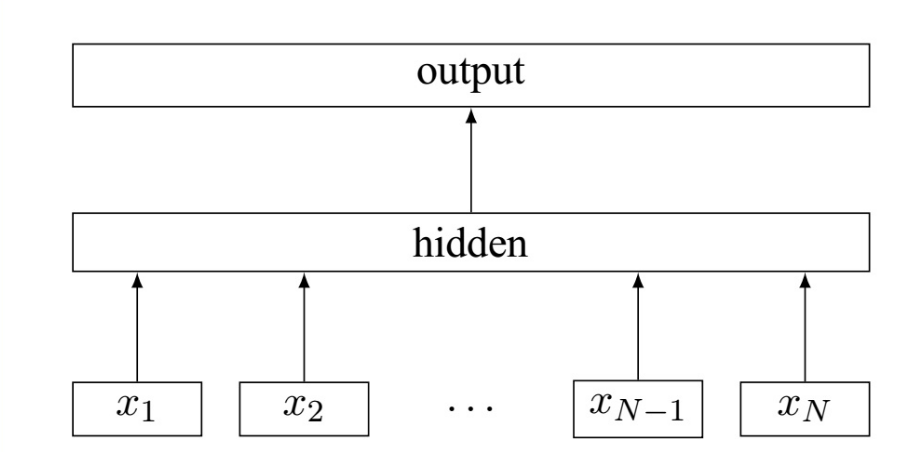
\includegraphics[width=8cm]{figures/fasttext_model_architecture.png}
	\caption{Model architecture of \emph{fastText} for a sentence with $N$ gram features $x_1,...,x_N$. The features are embedded and average to form the hidden variable.}
	\label{fig:fasttext}
\end{figure}

Figure \ref{fig:fasttext} is the model architecture of FastText, where the only difference between \emph{fastText} and CBOW is the subword model. Given a word \emph{where} and a character n-gram length equals to $3$. We first add special boundary symbols $<$ and $>$ at the beginning and end of words, then taking all its character ngrams --- where $\to$ <wh, whe, her, ere, re>, <where>. \\

The scoring function is then $s(w,c)=\sum_{g\in G_w}{z_g^{\top}v_c}$ 


\section{ELMo}
\textbf{E}mbeddings from \textbf{L}anguage \textbf{Mo}dels (ELMo) \citep{peters2018deep} attempts to resolve two challenges:
\begin{enumerate}
	\item complex characteristics of word use (e.g.,syntax and semantics)
	\item how these uses vary across linguistic contexts \\
\end{enumerate} 

\subsection{Bidirectional language models}

Given a sequence of $N$ tokens, ($t_1, t_2 , ..., t_N$ ), a forward language modeling the probability of $t_k$
$$p(t_1,t_2,...,t_N)=\prod_{k=1}^{N}{p(t_k|t_1,t_2,...,t_{k-1})}$$
whilst a backward model as 
$$p(t_1,t_2,...,t_N)=\prod_{k=1}^{N}{p(t_k|t_{k+1},t_{k+2},...,t_{N})}$$

A biLM combines both LMs and jointly maximizes the log likelihood as 
$$\sum_{k=1}^{N}{(\log{p(t_k|t_1,t_2,...,t_{k-1};\Theta_x,\Theta_{LSTM},\Theta_{s}) + p(t_k|t_{k+1},t_{k+2},...,t_{N};\Theta_x, \Theta_{LSTM},\Theta_s)})}$$ \\


\subsection{ELMo}

For each token $t_k$, a $L$-layer biLM computes a set of $2L+1$ representations
$$R_k = \{x_K^{LM}, \overrightarrow{h}_{k,j}^{LM}, \overleftarrow{h}_{k,j}^{LM} |j=1,...,L\}$$

ELMo collapses all layers in $R$ into a single vector, $ENMo_k=E(R_k;\Theta_{e})$.
In general, a task specific weighting of all biLM layers: 
$$ELMo_{k}^{task}=E(R_k;\Theta^{task})=\gamma^{task}\sum_{j=0}^{L}{s_j^{task}h_{k,j}^{LM}}$$
where $s^{task}$ are softmax-normalized weights and scalar $\gamma^{task}$ allows the task model to scale the entire ELMo vector.

\section{BERT}
The main contribution of \textbf{B}idirectional \textbf{E}ncoder \textbf{R}epresentation from \textbf{T}ransformer (BERT) are the follows:
\begin{itemize}
	\item demonstrate the importance of bidirectional pre-training for language representations, also \emph{in contrast to \citep{peters2018deep} which uses a shallow concatenation of independently trained left-to-right and right-to-left LMs.} 
	\item pre-trained representations eliminate the needs of many heavily-engineered task-specific architectures.
	\item bidirectional nature of the model is the single most important new contribution.
\end{itemize}

\subsection{Apply to Downstream Tasks}
Generally, there are two existing strategies for applying pre-trained language representations to down-stream tasks: \emph{feature-based} and \emph{fine-tuning}.

\begin{itemize}
	\item \textbf{Feature-based}: such as ELMo, uses tasks-specific architectures that include the pre-trained representations as additional features.
	\item \textbf{Fine-tuning}: such as Skip-gram, GPT and BERT, introduced minimal task-specific parameters, and is trained on the downstream  tasks by simply fine-tuning the pre-trained parameters.
\end{itemize}

\begin{figure}[htpb]
	\centering
	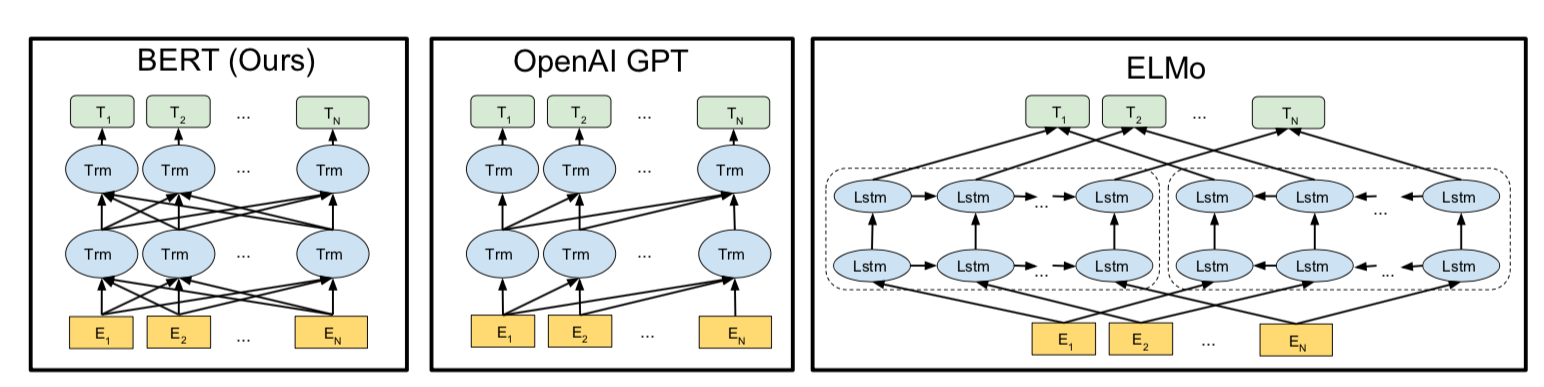
\includegraphics[width=\linewidth]{figures/diff_bert_gpt_emlo.png}
	\caption{Differences in pre-training model architectures. BERT uses a bidirectional Transformer. OpenAI GPT uses a left-to-right Transformer. ELMo uses the concatenation of independently trained left-to-right and right- to-left LSTM to generate features for downstream tasks. Among three, only BERT representations are jointly conditioned on both left and right context in all layers.}
	\label{fig:diff_bert_gpt_emlo}
\end{figure}

\subsection{Model Architecture}
\begin{itemize}
	\item \textbf{L}: the number of layers (Transformer block)
	\item \textbf{H}: the hidden size 
	\item \textbf{A}: the number of self-attention heads
\end{itemize}
BERT primarily report results on two model size:
\begin{itemize}
	\item \bolden{$\text{BERT}_{\text{BASE}}$}: L=12, H=768, A=12, Total Parameters=110M
	\item \bolden{$\text{BERT}_{\text{LARGE}}$}: L=24, H=2014, A-16, Total Parameters=340M
\end{itemize}
The difference between BERT, GPT and ElMo is shown visually in Figure \ref{fig:diff_bert_gpt_emlo}. Note that we often refer the bidirectional Transformer (left) as "Transformer encoder" while the left-context-only version (middle) is referred as a "Transformer decoder".

\subsection{Input Representation}
\begin{figure}[htpb]
	\centering
	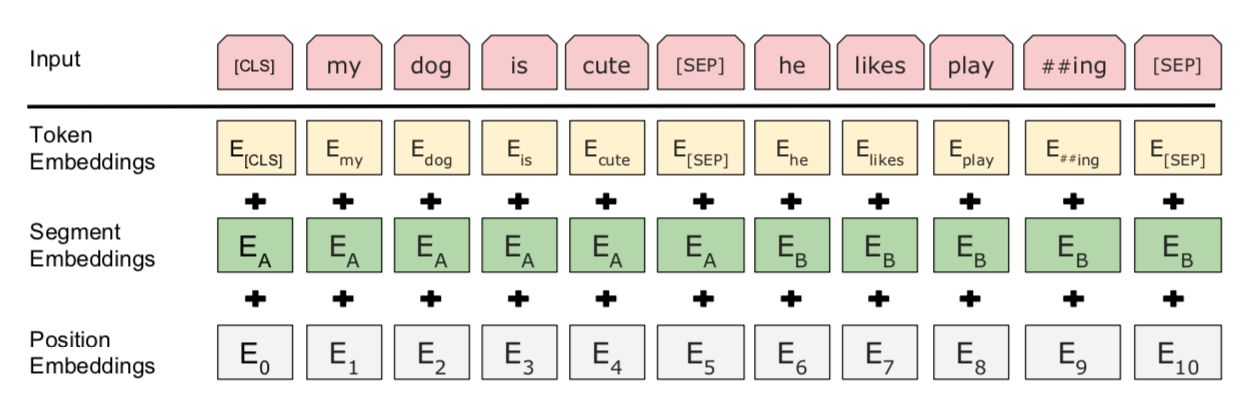
\includegraphics[width=\linewidth]{figures/bert_input_representation.png}
	\caption{BERT input representation. The input embeddings is the sum of the token embeddings, the segmentation embeddings and the position embeddings.}
	\label{fig:bert_input_representation}
\end{figure}
\begin{itemize}
	\item use WordPiece embeddings with a 30,000 token vocabulary.
	\item use learned positional embeddings with supported sequence lengths up to 512 tokens.
	\item sentences pairs are packed together into a single sequence, \emph{a "sentence" can be an arbitrary span of contiguous text, rather than an actual linguistic sentence}
	\item the first token of every sequence is al- ways the special classification embedding ([CLS]). The final hidden state (i.e., out- put of Transformer) corresponding to this token is used as the aggregate sequence representation for classification tasks. For non- classification tasks, this vector is ignored.
	\item sentences are differentiated in two ways. First, we separate them with a special token ([SEP]). Second, we add a learned sentence A embedding to every token of the first sentence and a sentence B embedding to every token of the second sentence.
\end{itemize}


\subsection{Pre-trained Tasks}
\subsubsection{Masked LM}
The final hidden vectors corresponding to the \textbf{masked tokens} are fed into an output softmax over vocabulary, as in standard LM. In all of experiments, 15\% of all WordPiece tokens in each sequence at random and then we perform the following procedure:
\begin{itemize}
	\item 80\% of the time: Replace the word with the [MASK] token, e.g., \emph{my dog is hairy $\to$ my dog is [MASK]}
	\item 10\% of the time: Replace the word with a random word, e.g., \emph{my dog is hairy $\to$ my dog is apple}
	\item 10\% of the time: Keep the word unchanged, e.g., \emph{my dog is hairy $\to$ my dog is hairy.} The purpose of this is to bias the representation towards the actual observed word.
\end{itemize}

\subsubsection{Next sentence prediction}
In order to train a model that understands sentence relationships which are beneficial to tasks like Question Answering (QA) and Natural Language Inference (NLI), a binarized \emph{next sentence prediction} task that can be trivially generated from any monolingual corpus. \\

Specifically, when choosing the sentences A and B for each pre-training example, 50\% of the time B is the actual next sentence that follows A, and 50\% of the time it is a random sentence from the corpus. 

\subsection{Ablation Studies}
\begin{enumerate}
	\item \textbf{No NSP}: A model which is trained using the “masked LM” (MLM) but without the “next sentence prediction” (NSP) task.
	\item \textbf{LTR \& No NSP}: A model which is trained using a Left-to-Right (LTR) LM, rather than an MLM
\end{enumerate}
The result of all variants of BERT is shown in Figure \ref{fig:bert_ablation_study}.
\begin{figure}[htpb]
	\centering
	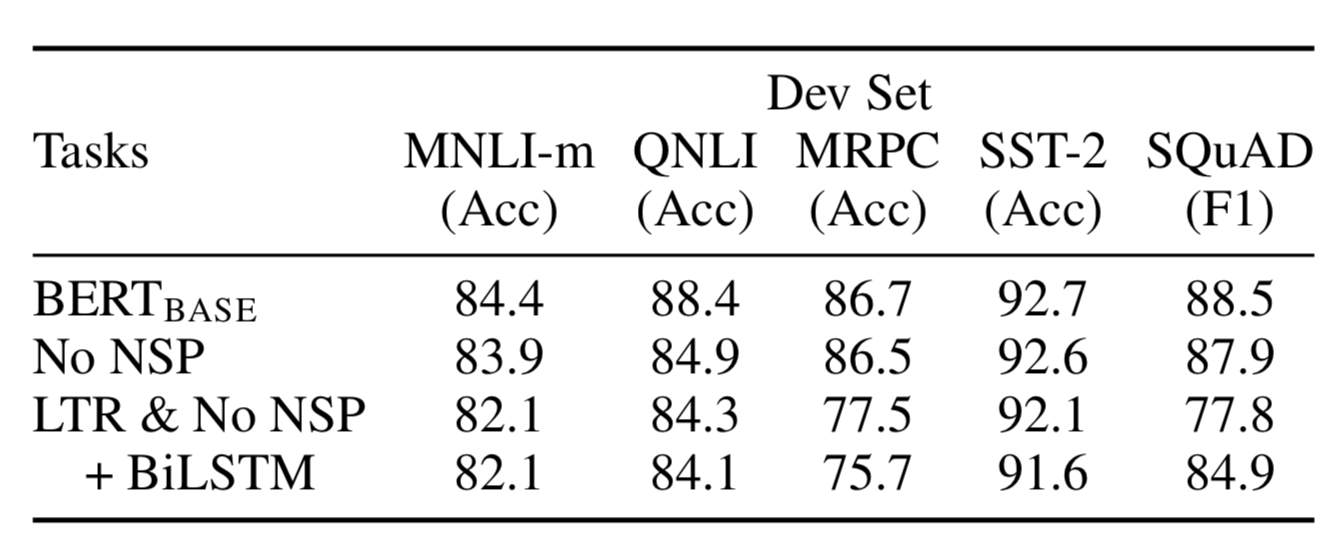
\includegraphics[width=\linewidth]{figures/bert_ablation_study.png}
	\caption{Ablation over the pre-training tasks using the BERTBASE architecture. “No NSP” is trained without the next sentence prediction task. “LTR \& No NSP” is trained as a left-to-right LM without the next sentence prediction, like OpenAI GPT. “+ BiLSTM” adds a randomly initialized BiLSTM on top of the “LTR + No NSP” model during fine-tuning.}
	\label{fig:bert_ablation_study}
\end{figure}


\chapter{Chinese Word Segmentation}
\section{Dictionary-Based Method}

\chapter{Neural Algorithms For Name Entity Recognition}
\section{LSTM-CRF Model}
A hybrid tagging architecture combined LSTMs and CRFs is presented here. The LSTMs part always adopts a bi-directional LSTM module, which take as input a sequence of vectors $(x_1, x_2,...x_n)$ and return another sequence $(h_1,h_2,...,h_n)$. The representation of a word using this model is obtained by concatenating its left and right context representations, $h_t=[\overrightarrow{h_t};\overleftarrow{h_t}]$.

\subsection{CRF Tagging Model}
\subsubsection{Why do we need a CRF Tagging Module?}
Considered a very simple --- but surprisingly effective --- tagging model is to use the $h_t$'s as features to make \textbf{independent} tagging decisions for each output $y_t$. Despite the model's success in simple problems like \textbf{POS tagging}, its independent classification decisions are limited when there are \textbf{strong dependencies across output labels}. \textbf{NER} is one such task, since the "grammar" that characterizes interpretable sequences of tags imposes several hard constraints (e.g., I-PER cannot follow B-LOC) that \textbf{impossible to model with independence assumptions}.

\subsubsection{Model detail}
Instead of modeling tagging decisions independently, we model $h_t$ jointly using a conditional random field. For an input sentence 
$$X=(x_1, x_2,...,x_n)$$
we consider $P$ to be matrix of scores output by the bi-directional LSTM network. $P$ is of size $n\times k$, where $k$ is the number of distinct tags, and $P_{i,j}$ corresponds to the score of the $j^{th}$ tag of the $i^{th}$ word in a sentence. For a sequence of predictions 
$$y=(y_1,y_2,...,y_n)$$
we define its score to be 
\begin{equation}
s(X,y)=\sum_{i=0}^{n}{A_{y_i,y_{i+1}}}+\sum_{i=1}^{n}{P_{i,y_i}}
\end{equation}
where $A$ is a matrix of transition scores such that $A_{i,j}$ represents the score of a transition from the tag $i$ to tag $j$. ($y_0$ and $y_n$ are the \emph{start} and \emph{end} tags of a sentence, that we add to the set of possible tags. $A$ is therefore a square matrix of size $k+2$) \\

\textbf{Note}: this part is actually very similar to the Hidden Markov Model(HMM), where $P$ is the \emph{emission matrix} and $A$ is the \emph{transmission matrix}, except that the scores are \textbf{unnormalized} which can not be formed as probabilities. \\

A softmax over all possible tag sequences yield a probability for the sequence $y$:
\begin{equation}
p(y|X)=\frac{e^{s(X,y)}}{\sum_{\tilde{y} \in Y_x {e^{s(X,\tilde{y})}}}}
\end{equation}
During \textbf{training}, we maximize the log-probability of the correct tag sequence:
\begin{equation}
\begin{split}
\log{(p(y|X))} & = s(X,y) - \log{(\sum_{\tilde{y} \in Y_x} {e^{s(X,\tilde{y})}})} \\
& = s(X,y) - \mathrm{logadd}_{\tilde{y} \in Y_x} {s(X,\tilde{y})}
\end{split}
\end{equation}
While \textbf{decoding}, we predict the output sequence that obtains the maximum score given by:
\begin{equation}
y^*=\mathrm{argmax}_{\tilde{y} \in Y_x}{s(X,\tilde{y})}
\end{equation}
Both the above the summation in training and maximum a posteriori sequence $y^*$ can be computed by using \textbf{dynamic programming}.

\subsubsection{Parameterization and Training}
The score associated with each tagging decision for each token ($P_{i,y}$) are defined to be the dot product between 

\begin{figure}[htpb]
	\centering
	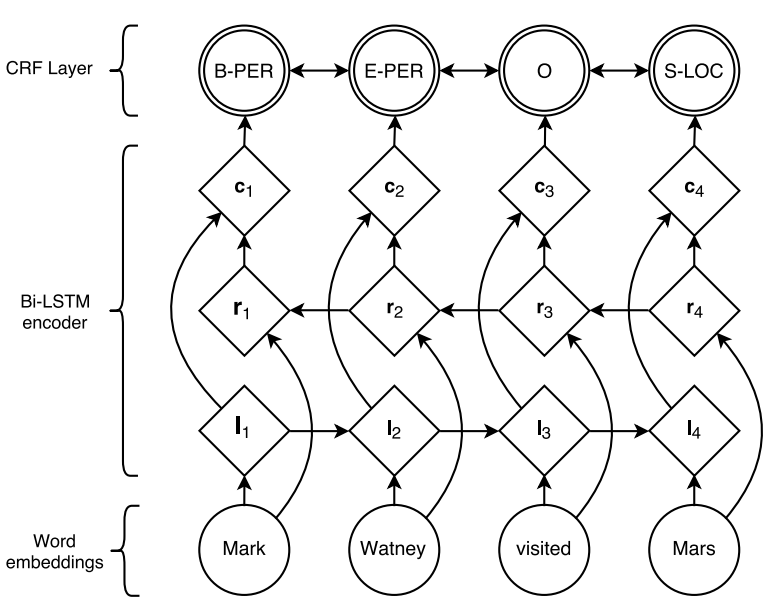
\includegraphics[width=10cm]{figures/lstm_crf.png}
	\caption{Main architecture of the LSTM-CRF network}
	\label{fig:boat1}
\end{figure}


\begin{itemize}
	\item \textbf{embedding of a word-in-context}: computed with a bi-directional LSTM, that is,  concatenating the forward and backward LSTM outputs and projecting onto  a layer whose \textbf{size is equal to the number of distinct tags} (instead of using the softmax output from the above mentioned layer). 
	\item \textbf{bigram compatibility scores $A_{y,y^{\prime}}$}: computed in the CRF layer.
\end{itemize}

\textbf{Note}: Adding a hidden layer between $c_i$ and CRF layer marginally improved the results.

\section{LSTM-CNN-CRF Model}
\begin{figure}[htpb]
	\centering
	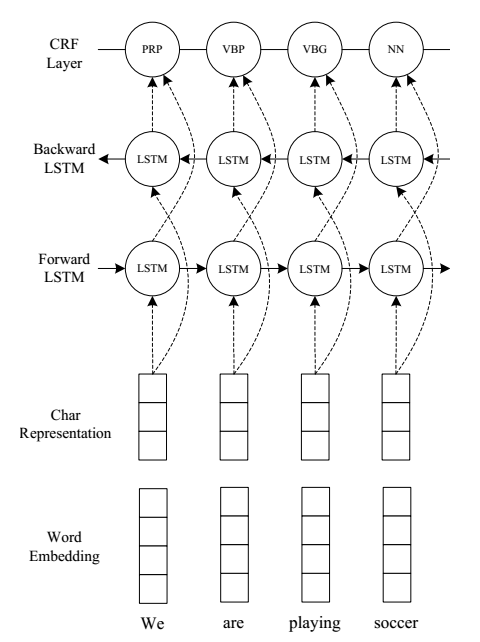
\includegraphics[width=10cm]{figures/lstm_cnn_crf.png}
	\caption{Main architecture of the LSTM-CNN-CRF network}
	\label{fig:boat1}
\end{figure}

\chapter{Topic Model}
In \emph{machine learning} and \emph{natural language processing}, a \textbf{topic model} is a type of statistic model of discovering the abstract "topics" that occur in a collection of documents.

\section{Probabilistic Latent Semantic Analysis}
\subsection{A Modern View of pLSA}
In order to better understand the intuition behind the model, we need to make some assumptions. First, we assume a topic $\phi_k$ is a distribution over a fixed size of vocabulary $V$. In the original pLSA model, this distribution is not explicitly specified but the form is Multinomial distribution. Thus, $\phi_k$ is essentially a vector that each element $\phi_{(k,w)}$ represents the probability that term $w$ is chosen by topic $k$, namely:
$$p(w|k)=\phi_{(k,w)}$$
and note $\sum_{w}^{V}\phi_{(k,w)}=1$. Secondly, we also assume that a document consists of multiple topics. Therefore, there is a distribution $\theta_{d}$ over a fixed number of topics $T$ for each document $d$. Similarly, original pLSA model does not have the explicit specification of this distribution but it is indeed a Multinomial distribution where each element $\theta_{(d,k)}$ in the vector $\theta_{d}$ represents the probability that topic $k$ appears in document $d$, namely
$$p(k|d)=\theta_{(d,k)}$$
and also $\sum_{k}^{T}\theta_{(d,k)}=1$. This is the prerequisite of the model. \\

pLSA can be considered as a \textbf{generative} model, where the generation process can be summarized as follows: \\

For each document $d$
\begin{itemize}
	\item For each token position $i$
	\begin{itemize}
		\item Choose a topic $z \sim $ Multinomial$(\theta_d)$
		\item Choose a term $w \sim $ Multinomial$(\phi_z)$
	\end{itemize}
\end{itemize}
and we can write the \textbf{probability a term} $w$ appearing at position $i$ in the document $d$ as follows:
\begin{equation}
	p(d_i=w|\Phi ,\theta_{d})=\sum_{z=k}^{T}{\phi_{(z,w)}\theta_{(d,z)}}
\end{equation}
and the joint probability of the whole dataset $\mathbf{W}$ is:
\begin{equation}
\begin{split} p(\mathbf{W}|\Phi,\Theta) & = \prod_d^D{\prod_i^{N_d}{\sum_{z=k}^T{\phi_{(z,w)}\theta_{(d,z)}}}} \\
& = \prod_d^D{\prod_w^{V}{(\sum_{z=k}^T{\phi_{(z,w)}\theta_{(d,z)}})^{n{(d,w)}}}} \end{split} \end{equation}
where $n(d,w)$ is the number of times term $w$ appearing in document $d$.

\section{Latent Dirichlet Allocation}
\subsection{The Dirichlet and its Relation to the Multinomial}
The Dirichlet distribution with parameter vector $\alpha$ of length $K$ is defined as 
\begin{equation}
Dirichlet(\theta;\alpha)=\frac{1}{B{(\alpha)}}\prod_{i=1}^{K}{\theta_i^{\alpha_i-1}}
\end{equation}
where $B(\alpha)$ is the multivariate Beta function, which can be expressed using gamma function as 
\begin{equation}
B(\alpha)=\frac{\prod_{i=1}^{K}{\Gamma{(\alpha_i)}}}{\Gamma{(\sum_{i=1}^{K}{\alpha_i})}}
\end{equation}



\chapter{Knowledge Graph}
\section{TransE}
\section{TransD}
\section{TransR}
\section{TransH}



\chapter{Question Answering}
\section{Summary}
Most question answering systems focus on \textbf{factoid questions}, two basic approaches towards this problem:
\begin{itemize}
	\item \textbf{IR-based question answering}
	\begin{itemize}
		\item[-] information retrieval techniques find relevant documents
		\item[-] \textbf{reading comprehension algorithms} to read these retrieved documents or passages
		\item[-] draw an answer directly from \textbf{spans of text}
	\end{itemize}
	\item \textbf{Knowledge-based question answering}
	\begin{itemize}
		\item[-] build a semantic representation of the query to the logical representation
		\item[-] use meaning representation to query databases of facts
	\end{itemize}
\end{itemize}

\begin{figure}[htpb]
	\centering
	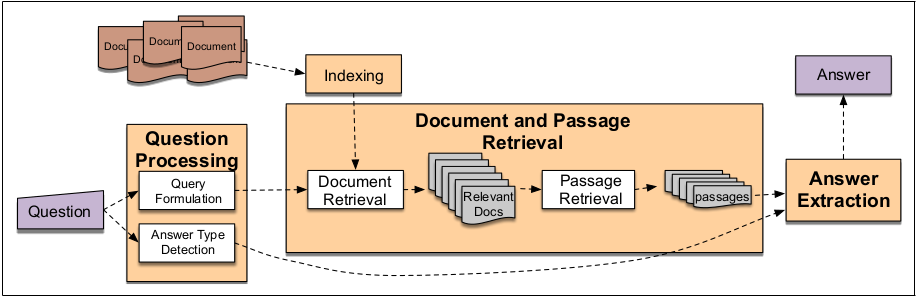
\includegraphics[width=\linewidth]{figures/ir_qa_overview.png}
	\caption{IR-based factoid question answering has three stages: question processing, passage retrieval, and
		answer processing.}
	\label{fig:boat1}
\end{figure}

\section{IR-based Question Answering}
\subsection{Question Processing}
Extract the \textbf{query}: the keyword to match potential documents, along with additional \textbf{features}:
\begin{itemize}
	\item \textbf{answer type}: the entity type (person, location, time, etc.) of the answer.
	\item \textbf{focus}: the string of words in the question that are likely to be replaced by the answer in any answer string found.
	\item \textbf{question type}: is this a definition question, a math question, a list question?
\end{itemize}


\textbf{Example}:
\begin{itemize}
	\item question: \emph{Which US state capital has the largest population?}
	\item query: \emph{US state capital has the largest population}
	item answer type: \emph{city}
	\item focus: \emph{state capital}
\end{itemize}

\subsection{Query Formulation}
\textbf{Query formulation} is a task of creating a query -- a list of tokens -- to send to information retrieval system. For QA from smaller	sets of documents, \textbf{tf-idf cosine matching} and \textbf{query expansion} may be helpful. \\
\textbf{Query reformulation} rephrases the question to
make it look like a substring of possible declarative answers. \emph{"when was the laser invented?"} $\to$\emph{"the laser was invented"}

\subsection{Answer Types}
Some systems make use of \textbf{question classification} to find the answer type. Each question can be labeled with a tag.

\begin{itemize}
	\item \textbf{rule-based}:
	\item \textbf{supervised learning}:
\end{itemize}

\subsection{Document and Passage Retrieval}
1. IR engine ranks the documents by their relevance to the query. \\
2. QA systems divide the top n documents into smaller passages such
as sections, paragraphs, or sentences.\\
3. Filter the passages by running answer type or name entity classification. \\
4. Supervised learning algorithms fully rank the rest passages with features like:
\begin{itemize}
	\item The number of \textbf{named entities} of the right type in the passage
	\item The number of \textbf{question keywords} in the passage
	\item The longest exact sequence of \textbf{question keywords} that occurs in the passage
	\item The rank of the document from which the passage was extracted
	\item The \textbf{proximity} of the keywords from the original query to each other
	\item The number of \textbf{n-grams} that \textbf{overlap} between the passage and the question
\end{itemize} 

\subsection{Answer Extraction}
In this step, a specific answer is extracted from the passage. This task is commonly modeled by \textbf{span labeling}: given a passage, identifying the \textbf{span} of the text which constitutes an answer.


\chapter{Machine Translation}
\section{Transformer}
The full architecture of a Transformer Seq2Seq model is shown in Figure \ref{fig:transformer}
\begin{figure}[htpb]
	\centering
	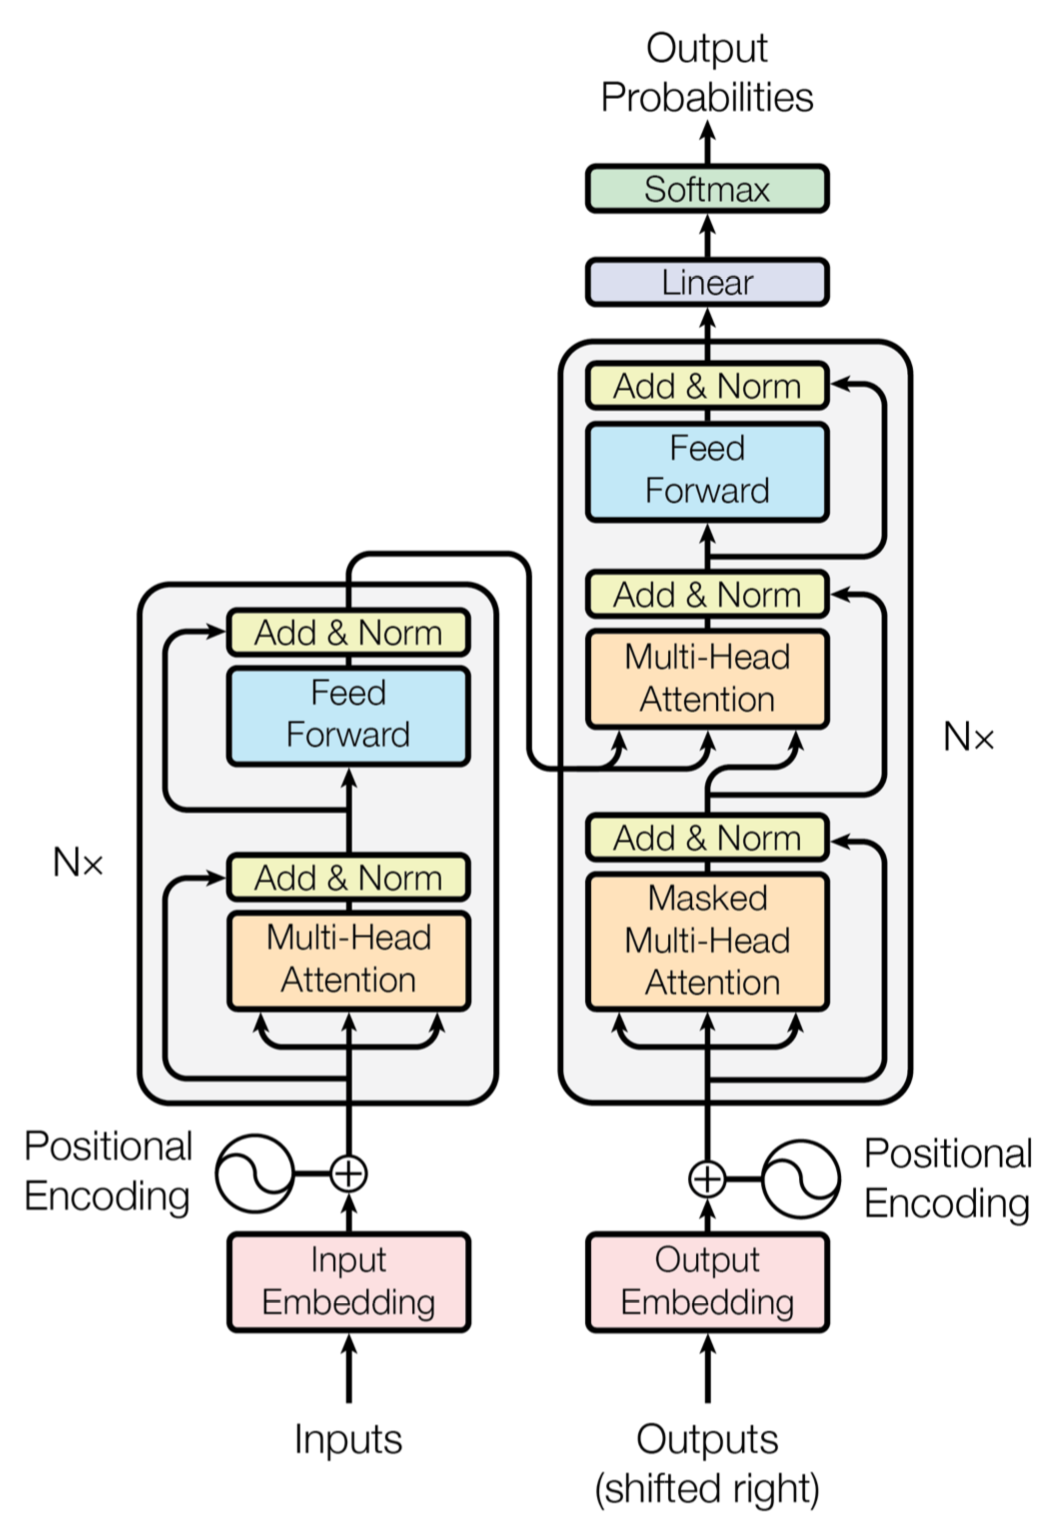
\includegraphics[width=10cm]{figures/transformer.png}
	\caption{The Transformer - model architecture.}
	\label{fig:transformer}
\end{figure}


\subsection{Attention}
\begin{figure}[htpb]
	\centering
	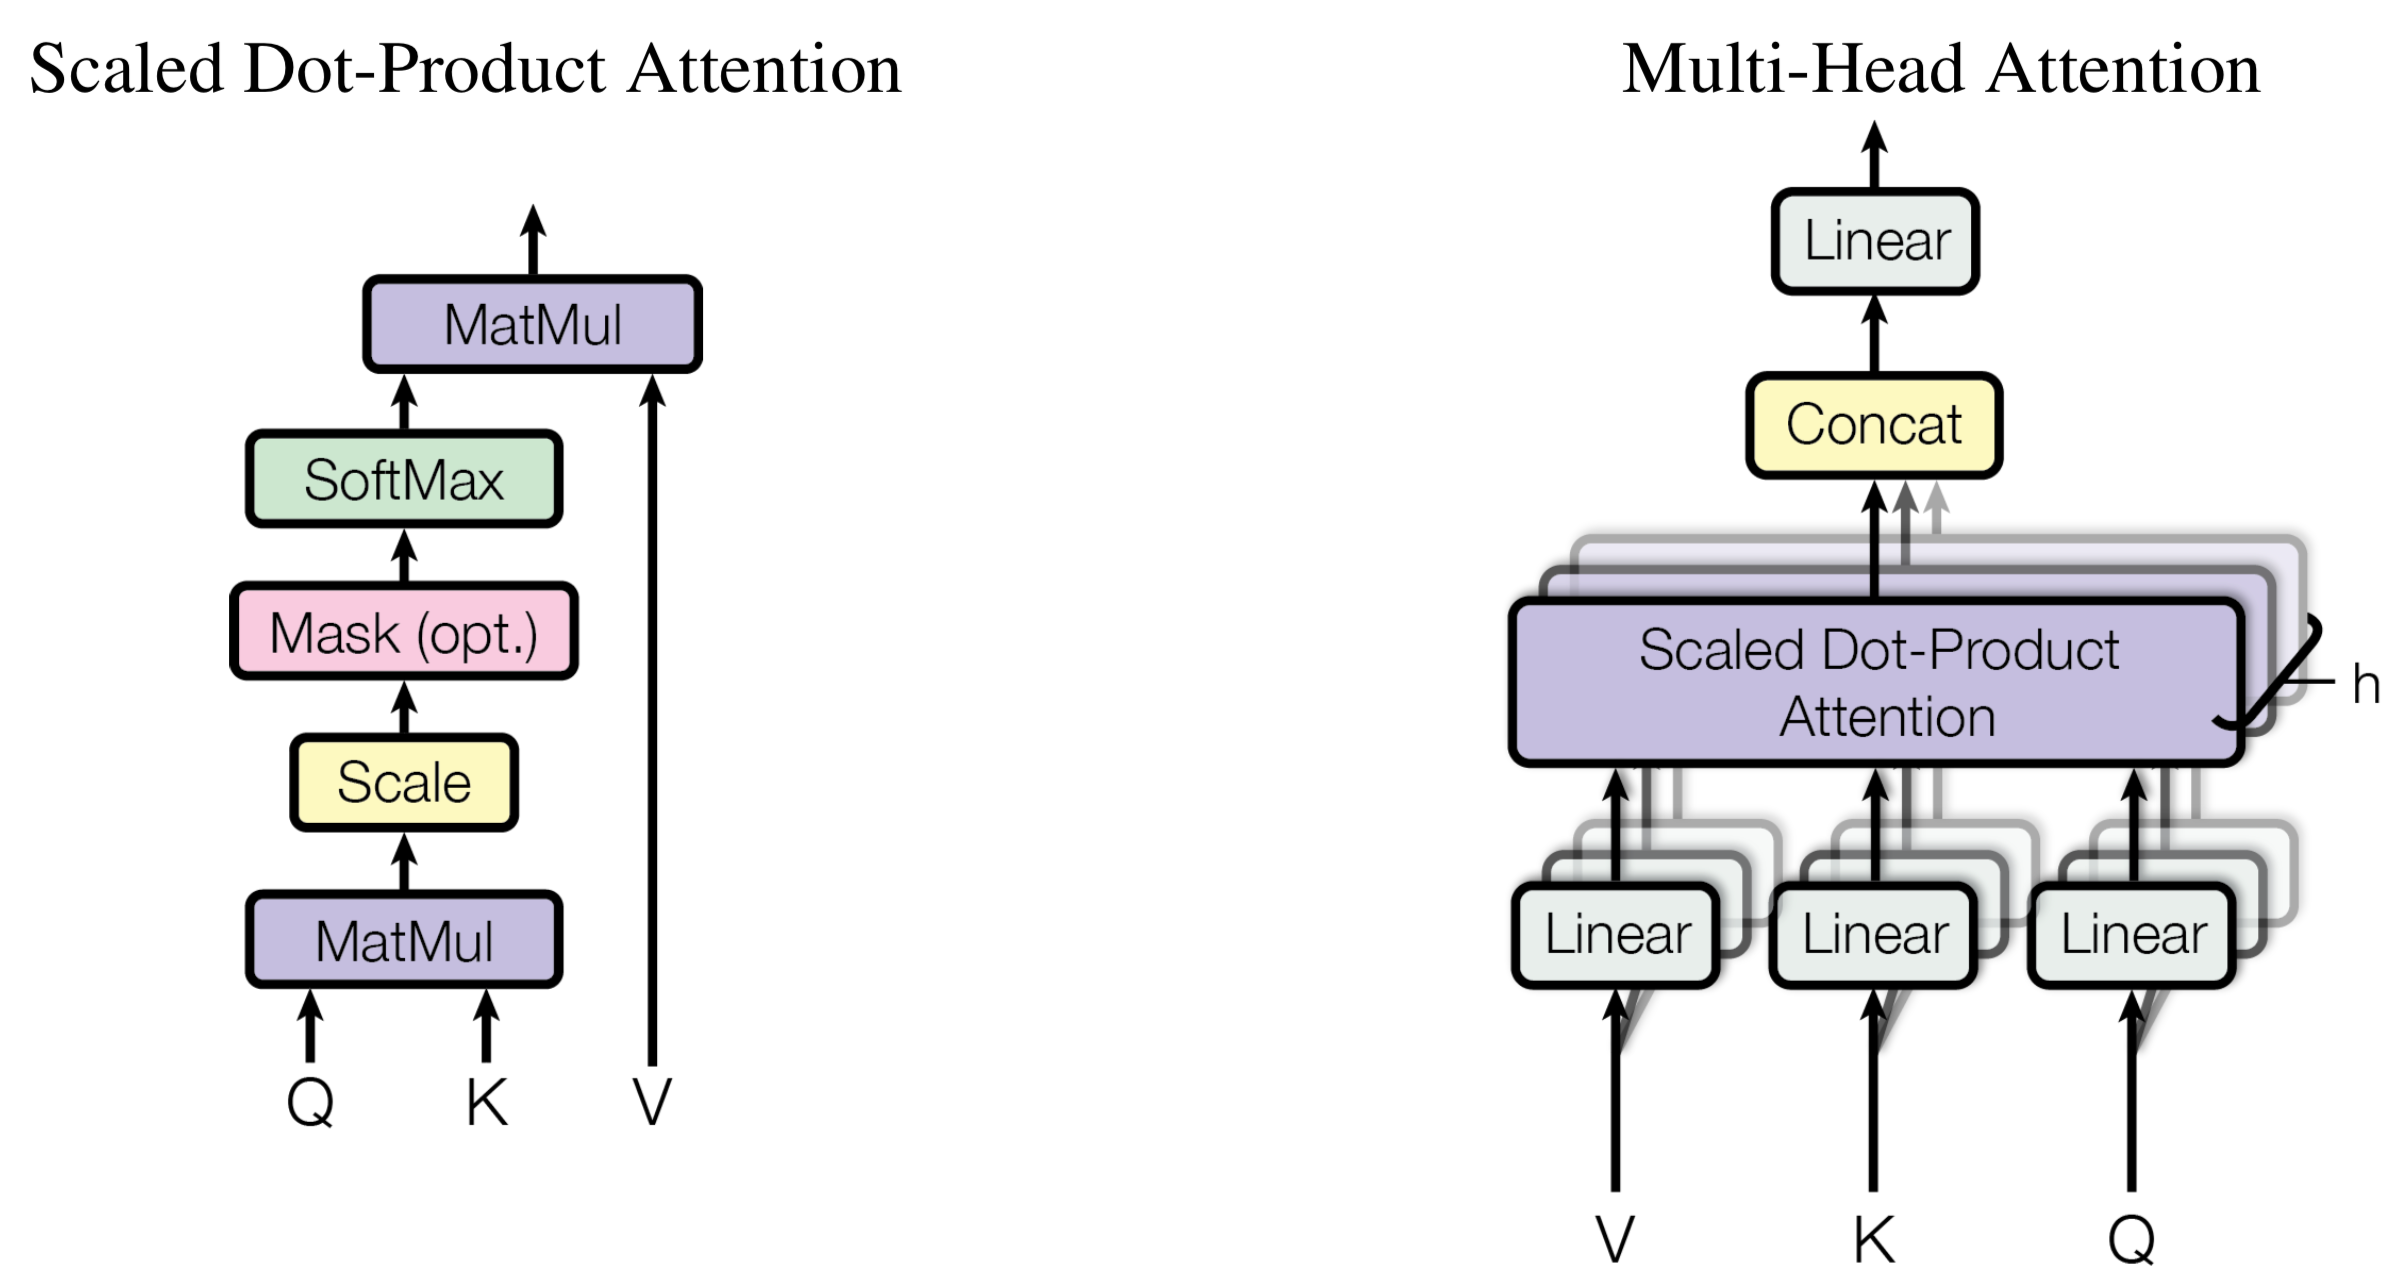
\includegraphics[width=\linewidth]{figures/attention_transformer.png}
	\caption{(left) Scaled Dot-Product Attention. (right) Multi-Head Attention consists of several attention layers running in parallel.}
	\label{fig:boat1}
\end{figure}

\subsubsection{Scaled dot-product attention}
An attention function can be described as mapping a \textbf{query} ($Q \in \mathbb{R}^{n\times d_k}$) and a set of \textbf{key-value} pairs ($K \in \mathbb{R}^{n\times d_k} $ and $V \in \mathbb{R}^{m \times d_v}$) to an output, where the query, keys, values, and output are packed matrix of a set of vectors. Which we can think the attention layer \bolden{maps a $n\times d_k$ sequence $Q$  into a new sequence $n \times d_v$}. \\

The output is computed as a \textbf{weighted sum} of the values, where the weight assigned to each value is computed by a compatibility function of the query with the corresponding key.
\begin{equation}
\text{Attention}{(Q,K,V)}= \text{softmax}{(\frac{QK^{\top}}{\sqrt{d_k}})}
\end{equation}
where $d_k$ is the dimension of $K$, for large values of $d_k$, the dot products grow large in magnitude, pushing the softmax function into regions where it has extremely small gradients.
\subsubsection{Multi-Head attention}
Instead of performing a single attention function, we found it beneficial to linearly project the queries, keys and values $h$ times with different learned linear projections to $d_k$, $d_k$ and $d_v$ dimensions.
\begin{equation}
\begin{split}
& \text{MultiHead}(Q,K,V)=\text{Concat}(\text{head}_1, ...,\text{head}_n) W^O \\
& \text{where } \text{head}_i = \text{Attention}(QW_i^Q, KW_i^K, VW_i^V)  \\
\end{split}
\end{equation}
Where the projections are parameter matrices $W_i^Q \in \mathbb{R}^{d_{model}\times d_k}$,  $W_i^K \in \mathbb{R}^{d_{model}\times d_k}$,  $W_i^V \in \mathbb{R}^{d_{model}\times d_v}$ and $W^O \in \mathbb{R}^{hd_v \times d_{model}} $.

\subsection{Position-wise Feed-Forward Network}
Each of the layers contains a 1-d convolutional network with kernel size $1$ (applied to each position separately and identically)
\begin{equation}
\text{FFN}(x) = \text{max}(0, xW_1+b_1)W_2+b_2
\end{equation}
For example, given a sentence with token $x_1, x_2,..., x_n$, for each $x_i$, we apply the above formula with the same weight and bias.

\subsection{Embeddings and Softmax}

\subsection{Positional Embedding}

\section{Learning From Monolingual Data}
\subsection{Back Translation}
\begin{enumerate}
\item Trains an intermediate system on the parallel data to translate the \textbf{target} monolingual data into
the \textbf{source} language. 
\item The synthetic parallel corpus is then
simply added to the real bitext in order to re-train from the \textbf{source}
to the \textbf{target} language.
\end{enumerate}

\citep{edunov2018understanding}

\section{Learning From Multilingual Data}
\subsection{One-to-Many}
\citep{wang2018three} proposed three strategies to improve one-to-many multilingual translation based on \textbf{transformer Seq2Seq}:
\begin{itemize}
	\item \textbf{Special Label Initialization} adds a special token (e.g. \textbf{2fr}) at the \textbf{beginning of the decoder} instead of normally adding special token (e.g. \textbf{en2fr}) at the end of the source sentence. 
	\item \textbf{Language-dependent Positional Embedding}
	\begin{itemize}
		\item \emph{Fixed embedding method}: introduce trigonometric functions with different orders or offsets on decoder to distinguish different target languages.
		\item \emph{Dynamic embedding method}: equip the tar- get inputs by embedding the absolute position of different languages separately.
	\end{itemize}
	\item \textbf{Shared and Language-dependent Hidden Units per Layer}: For instance, as shown in Figure \ref{fig:wang2018three_shared_layer}, in training step for one target language (tar-1), we tune the shared units and the language-dependent units of tar-1, and mask out other parts. In decoding step, we only use the shared and language-dependent hid- den units of target language tar-1 to predict translation results.
\end{itemize}

\begin{figure}[htpb]
	\centering
	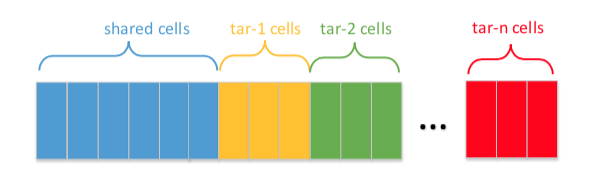
\includegraphics[width=8cm]{figures/wang2018three.png}
	\caption{The hidden units of decoder network. Blue part represents the shared units, and yellow, green and red parts denotes different language-dependent units respectively.}
	\label{fig:wang2018three_shared_layer}
\end{figure}

\section{Simultaneous Translation}
\subsection{"Wait-\emph{k}" Model}
\citep{ma2018stacl} proposed a strategy to achieve this aim on ordinary sequence modeling networks (e.g. RNN and Transformer). Conventional methods models the target token with the following probability 
\begin{equation}
p(\mathbf{y}|\mathbf{x})=\prod_{t=1}^{|\mathbf{y}|}{p(y_t|\mathbf{x}, \mathbf{y}_{<t})}
\end{equation}
while "wait-k" method modifies the above formula as follows, which means that \bolden{decoder always decodes a $t$ target token by only observing at most  $k+t-1$ source tokens.}
\begin{equation}
p(\mathbf{y}|\mathbf{x})=\prod_{t=1}^{|\mathbf{y}|}{p(y_t|\mathbf{x}_{\le g(t)}, \mathbf{y}_{<t})}
\end{equation}
\begin{equation}
g(t)=
\left\{
\begin{array}{lr}
k+t-1 &  t < |x| - k\\
|x|& otherwise  
\end{array}
\right.
\end{equation}

\subsubsection{Simultaneous translation with Transformers}
The encoder of Transformer works in a self-attention fashion and takes an input sequence $\mathbf{x}$, and produces a new sequence of hidden states $\mathbf{z}=(x_1,...,z_n) $. Specifically, in the self-attention module, a \emph{self-attention weight} $\alpha_{ij}$ is calculated with $\alpha_{ij}= \frac{e_{ij}}{\sum_{l=1}^{n}{e_{ij}}}$.

In "wait-k" method, we modify the "weight" as $\alpha_{ij}= \frac{e_{ij}}{\sum_{l=1}^{t+k}{e_{ij}}}$ where for each translation time step $t$, the self-attention layer in encoder only allows each word attend to it's prefix.
\subsubsection{Context caching}
Due to the nature of self0-attention, each time the translation step increments from $t$ to $t+1$, every word which is prior to the new word $k+t+1$ on the source needs to \textbf{adjust} it's existing representation to absorb the new word's information. Therefore, \bolden{the source context stores a list of context vectors representing the tokens in source sequence at each time step $t$ }.
 
\subsubsection{Refinements: wait-k with Catchup}
The decoder of proposed “wait-k” process is always k words behind the incoming source stream. From the user perspective, all the previous words are decoded in a one-by-one fashion while \textbf{the last k words are shown at one time on the screen} (shown in Figure \ref{fig:stacl_catchup}) which is not user-friendly (especially when source language and target language have a big gap in length). The solution is to \bolden{replace $g(t)$ with a more flexible $g_c(x)$}
\begin{equation}
g(t)=
\left\{
\begin{array}{lr}
k+t-1 -c_t & 1 \le t < |x| - k\\
|x|& |x| - k ]le t 
\end{array}
\right.
\end{equation}
where $c_t$ increases by one when $t=3\times c_t$.s
\begin{figure}[htpb]
	\centering
	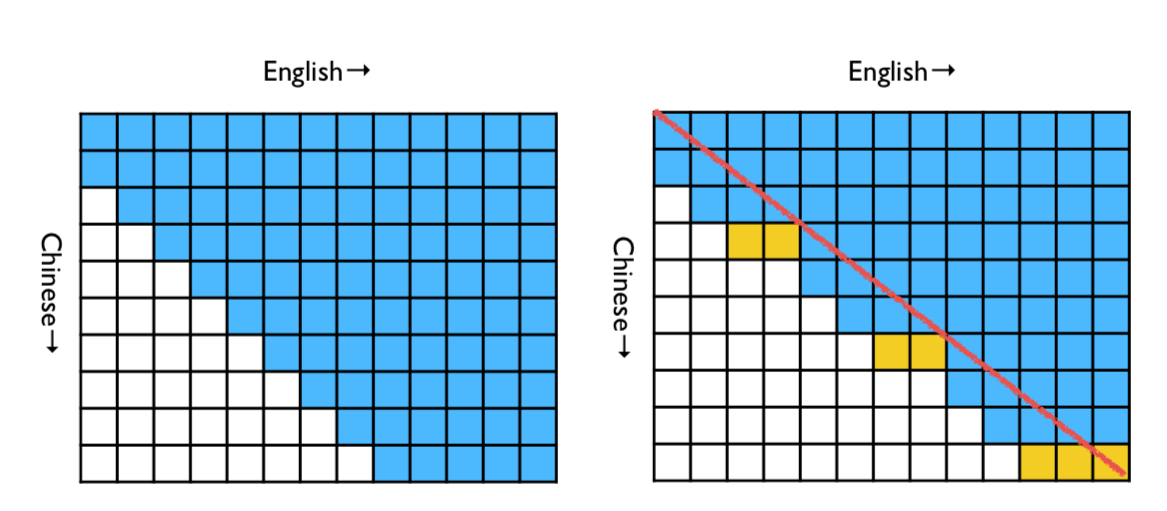
\includegraphics[width=\linewidth]{figures/stacl_catchup.png}
	\caption{Regular "wait-k" process on the left side. Catchup strategy on the right side. There two words less at the last translation step.}
	\label{fig:stacl_catchup}
\end{figure}
%----------------------------------------------------------------------------------------
%	BIBLIOGRAPHY
%----------------------------------------------------------------------------------------

\part{Deep Learning}

\chapter{Recurrent Neural Network}

\chapter{Improving Neural Networks}
\section{Batch Normalization}
\subsection{Internal Covariate Shift}
Internal covariate shift reduces the network learning efficiency since the \emph{the change in the distributions of layers need to continuously adapt to the new distribution}.

\subsubsection{Covriate shift extended to sub-network}
Consider a network computing 
$$l=F_2{(F_1{(u,\Theta_1)},\Theta_2)}$$
where $F_1$ and $F_2$ are arbitrary transformations, and the
parameters $\theta_1$, $\theta2$ are to be learned so as to minimize
the loss $l$.
where $F_1$ and $F_2$ are arbitrary transformations, and the parameters $\Theta_1$, $\Theta_2$ are to be learned so as to minimize the loss $l$. Learning $\Theta_2$ can be viewed as if the inputs $x=F_1{(u,\Theta_1)}$ are fed into the sub-network. $l=F_2{(x, \Theta_2)}$, thus a gradient step is exactly equivalent to that for a stand-alone network $F_2$ with input $x$. 

\textbf{As it is advantageous for the distribution of x to remain fixed over time, then $\mathbf{\Theta_2}$ does not have to readjust to compensate for the change in the distribution of x}.

\subsubsection{Help training process}
Consider a layer with a sigmoid activation function, as $|x|$ increases, $g^{'}{(x)}$ tends to zero. In practice, the saturation problem and the resulting vanishing gradients are amplified as the network depth increases. If we could ensure that \textbf{the distribution of nonlinearity inputs remains more stable as the network trains, then the optimizer would be less likely to get stuck in the saturated regime, and the training would accelerate}.

\subsection{Towards Reducing Internal Covariate Shift}
Let $x$ be a layer input, treated as a vector, and $\chi$ be the set of these inputs over the training data set. The normalization can then be written as a transformation
$$\hat{x}=\mathrm{Norm}{(x, \chi)}$$ which depends not only on the given \textbf{training example} $x$, but also on \textbf{all example} $\chi$. For backpropagation, we would need to compute the Jacobians
\begin{equation}
\frac{\partial{\mathrm{Norm}{(x,\chi)}}}{\partial{x}}, \frac{\partial{\mathrm{Norm}{(x,\chi)}}}{\partial{\chi}}
\end{equation} 

\subsubsection{Why not ignore the latter part?}
Ignoring the latter term would lead to the explosion. For example, consider a layer
with the input $u$ that adds the learned bias $b$, and normalizes the result by subtracting the mean of the activation computed over the training data: $\hat{x}=x-\mathbb{E}[x]$ where $x=u+b$, $\chi=\{x_1,...,x_N\}$ and $\mathbb{E}[x]=\sum_{i=1}^{N}x_i$.
 
If a gradient descent ignores the dependence of $\mathbb{E}[x]$ on $b$:
\begin{equation}
\begin{split}
	& b \leftarrow b + \Delta{b} \\
    & b \propto -\partial{l} / \partial{\hat{x}}
\end{split}
\end{equation}
Then 
$$u+(b + \Delta{b})-\mathbb{E}{(u+(b + \Delta{b}))}=u+b-\mathbb{E}{[u+b]}$$
The combination of the update to $b$ and subsequent change in normalization led to no change in the output of the layer nor the loss. As the training continues, \textbf{$\mathbf{b}$ will grow indefinitely} while the \textbf{loss remains fixed}. This problem can get worse if the normalization not only centers but also scales the activations.
\subsubsection{Simplification}  
The full whitening of each layer's inputs is costly (requires computing the covariance matrix $\mathrm{Cov}[X]=\mathbb{E}_{x\in \chi}{XX^\top}-\mathbb{E}{[X]}\mathbb{E}{[X]}^\top$ and its inverse square root, to produce the whitened activation) and not everywhere differentiable.
\begin{enumerate}
	\item \textbf{normalize each scalar feature independently} instead of whitening the features in layer inputs and outputs jointly, by making it have the mean of zero and variance of $1$. For a layer with $d$-dimensional input $x=(x^{(1)}...x^{(n)})$, we will normalize each dimension 
	$$\hat{x}^{(k)}=\frac{x^{(k)}-E{[x^{(k)}]}}{\sqrt{\mathrm{Var}{[x^{(k)}]}}}$$ where the expectation and variance are computed over the training data set.
	
	
	\item In the batch setting where each training step use \textbf{mini-batches} in stochastic gradient training instead of the whole training set.
\end{enumerate}

\subsubsection{Preserve the network capacity}
Noted that simply normalizing each input of a layer may change what the layer can represent. In order to maintain the \textbf{network capacity}, we make sure that \emph{the transformation inserted in the network can represent the identity transform}.

To accomplish this, we introduce, for each activation $x^{(k)}$, a pair of parameters $\gamma^{(k)}$, $\beta^{(k)}$, which scale and shift the normalized value:
$$y^{(k)}=\gamma^{(k)}\hat{x}^{(k)}+\beta^{(k)}$$
These parameters are learned along with the original
model parameters, and restore the representation power
of the network. Indeed, by setting $\gamma^{(k)} = \sqrt{\mathrm{Var}{[x^{(k)}]}}$ and
$\beta^{(k)} = \mathbb{E}[x^{(k)}]$, we could recover the original activations,
if that were the optimal thing to do.

\subsection{Training Algorithm}
\begin{figure}[htpb]
	\centering
	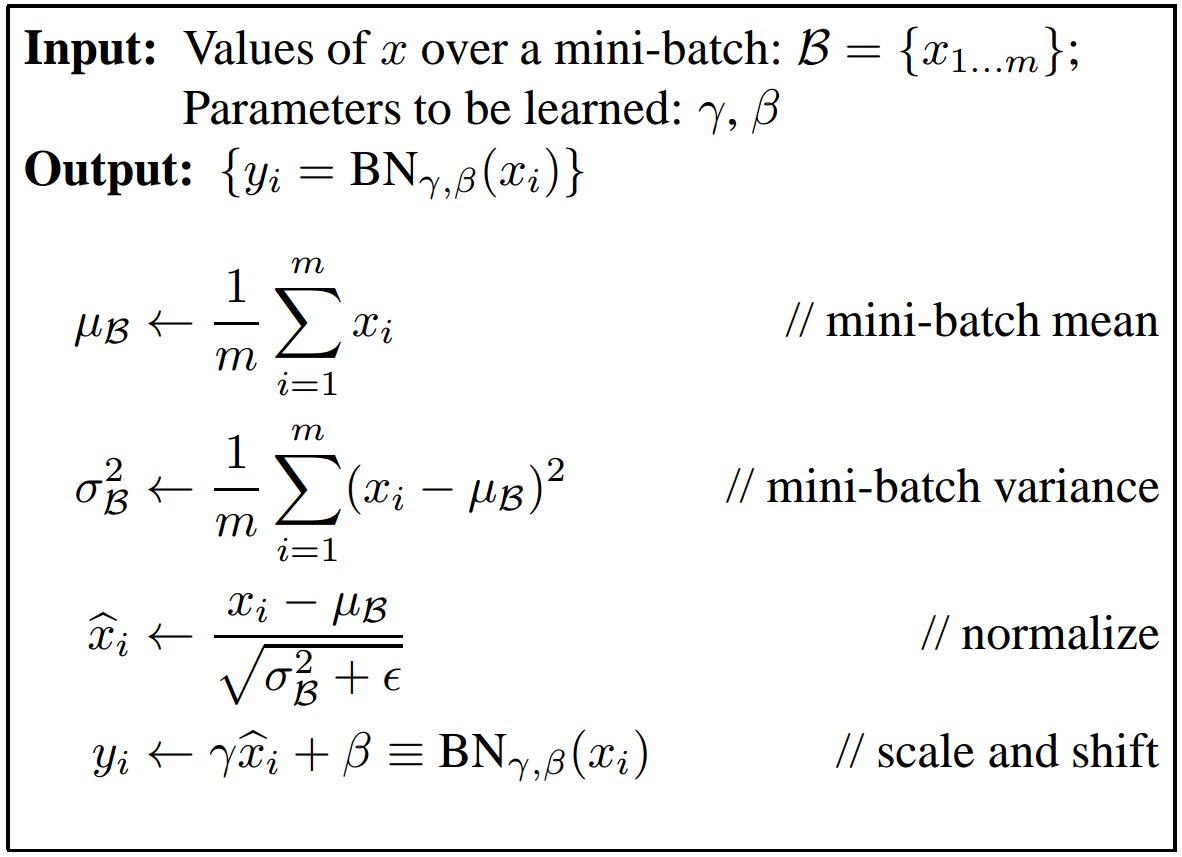
\includegraphics[width=10cm]{figures/bn_algorithm.png}
	\caption{Batch Normalizing Transform, applied to
activation $x$ over a mini-batch.}
	\label{fig:boat1}
\end{figure}
Each normalized activation $\hat{^{(k)}}$ can be viewed as an input to a sub-network composed of the linear transform $y^{(k)}=\gamma^{(k)}\hat{x}^{(k)}+\beta^{(k)}$, followed by the other processing done by the original network. 

\subsection{Inference}
The normalization of activations that
depends on the mini-batch allows efficient training, but is
neither necessary nor desirable during inference.

\begin{figure}[htpb]
	\centering
	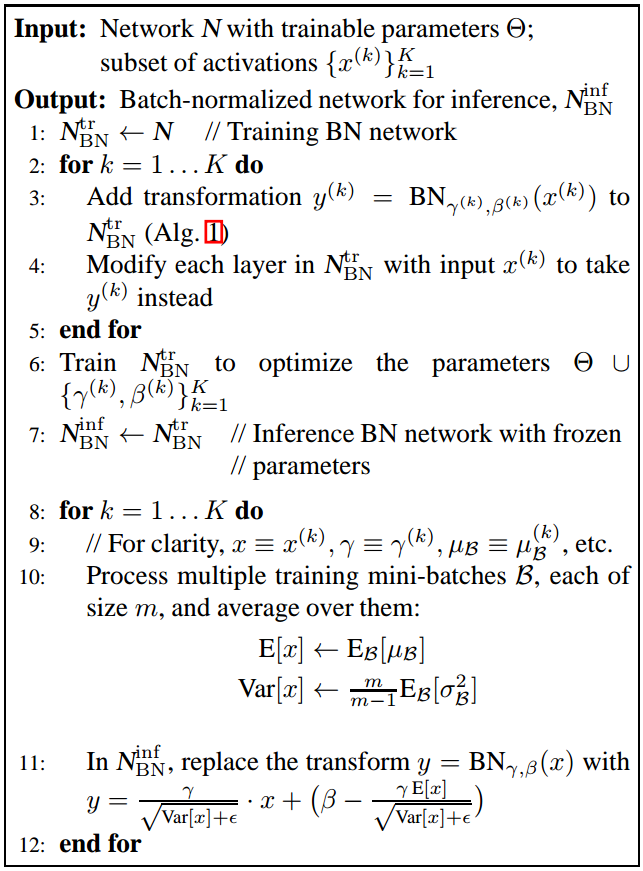
\includegraphics[width=\linewidth]{figures/bn_inference.png}
	\caption{Batch normalization inference}
	\label{fig:boat1}
\end{figure}
Once the network has been trained, we use the
normalization
$$\hat{x}=\frac{x-\mathbb{E}{[x]}}{\sqrt{\mathrm{Var}{[x]}+\epsilon}}$$
using the population, rather than mini-batch, statistics. Neglecting $\epsilon$, these normalized activations have the same mean $0$ and variance $1$ as during training. We use the unbiased variance estimate $\mathrm{Var}{[x]} = \frac{m}{m-1} \times E_{\beta}{[\sigma_{\beta}^2]}$, where
the expectation is over training mini-batches of size $m$ and $\sigma_{\beta}^2$ are their sample variances. 

Using moving averages instead, we can track the accuracy of a model as it trains.
Since the means and variances are fixed during inference,
the normalization is simply a linear transform applied to
each activation. It may further be composed with the scaling by $\gamma$ and shift by $\beta$, to yield a single linear transform
that replaces $\mathrm{BN}(x)$.

\section{Layer Normalization}
\subsection{Reasons Behind Layer Normalization}
The several drawbacks of \emph{batch normalization} remain as 
\begin{itemize}
	\item Batch normalization requires running averages of the summed input statistics. However, the summed inputs to the recurrent neurons in a recurrent neural network (RNN) often vary with the length of the sequence, so applying batch normalization to RNNs appears to \textbf{require different statistics for different time-steps}. 
	\item Batch normalization \textbf{cannot be applied to online learning tasks} or to extremely large distributed models where the \textbf{minibatches have to be small}.
\end{itemize}
\subsection{Method}
We compute the layer normalization statistics over all the hidden units in the same layer as follows:
\begin{equation}
\begin{split}
& \mu^l=\frac{1}{H} \sum_{i=1}^{H}{\alpha_{i}^{l}} \\
& \sigma^l = \sqrt[]{\frac{1}{H} \sum_{i=1}^{H}{(\alpha_{i}^{l}-\mu^l)^2}} \\
\end{split}
\end{equation}
where $H$ denotes the number of hidden units in a layer, note that the difference between \emph{layer normalization} and \emph{batch normalization} is that all the hidden units in a layer share the same normalization terms $mu$ and $\sigma$, but different training cases have different normalization terms. 


\section{Residual Network}
Denoting the desired underlying mapping as $\mathcal{H}{x}$, we let the stacked nonlinear
layers fit another mapping of $\mathcal{F}{(x)}=\mathcal{H}{(x)}-x$. The original mapping is recast into $\mathcal{F}{(x)}+x$. We hypothesize that it
is easier to optimize the residual mapping than to optimize
the original, unreferenced mapping. To the extreme, if an
identity mapping were optimal, \emph{it would be easier to push
the residual to zero than to fit an identity mapping by a stack of nonlinear layers}.
\begin{figure}[htpb]
	\centering
	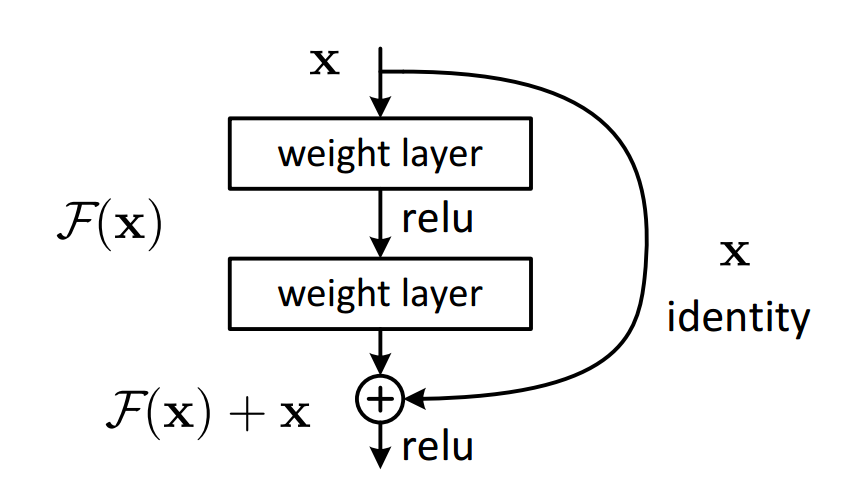
\includegraphics[width=8cm]{figures/resnet.png}
	\caption{Residual learning: a building block.}
	\label{fig:boat1}
\end{figure}
\subsection{Residual Learning}





\chapter{Unsupervised Learning}
\section{Generative Adversarial Nets}
\subsection{Adversarial Nets}
\begin{itemize}
	\item \textbf{Generator}: $p_z(z)$ $\to$ $G(z;\theta_g)$ $\to$ $p_g$
	\begin{itemize}
		\item $p_z(z)$: prior on input noise variables
		\item $G(z;\theta_g)$: a differentiable function represented by a multilayer perceptron with parameters $\theta_g$
		\item $p_g$: generator's distribution
	\end{itemize}
	\item \textbf{Discriminator}: $p_g$ $\to$ $D(x;\theta_d)$
	\item \textbf{Objective}: $D$ and $G$ play the following two-player minimax game with value function $V(G, D)$
	$$\min_G\max_D{V(D,G)}=\mathbb{E}_{x\sim p_{data}{(x)}}[\log{D(x)}]+\mathbb{E}_{z\sim p_{z}{(z)}}[\log{(1-D(G(z))))}]$$
\end{itemize}
\subsection{Algorithm}
\textbf{for} number of training iterations \textbf{do}\\
\indent \textbf{for} k steps \textbf{do} 
\begin{itemize}[leftmargin=+0.5in]
	\item Sample minibatch of $m$ noise samples $\{z^{(1)},..., z^{(m)}\}$ from noise prior $p_g{(z)}$.
	\item Sample minibatch of $m$ examples $\{x^{(1)},..., x^{(m)}\}$ from data generating distribution $p_{data}{(x)}$
	\item Update the discriminator by \textbf{ascending} its stochastic gradient:
	$$\nabla_{\theta_d}{\frac{1}{m}\sum_{i=1}^{m}{ [\log{D(x^{(i)})}+\log{(1-D(G(z^{(i)})))}]}}$$
\end{itemize}
\indent\indent \textbf{end for} 
\begin{itemize}
	\item Sample minibatch of m noise samples $\{z^{(1)},..., z^{(m)}\}$ xfrom noise prior $p_g{(z)}$.
	\item Update the generator by \textbf{descending} its stochastic gradient:
		$$\nabla_{\theta_g}{\frac{1}{m}\sum_{i=1}^{m}{\log{(1-D(G(z^{(i)})))}}}$$
\end{itemize}
\textbf{end for}
\subsection{Wasserstein GAN}

\section{Variational Auto-Encoder}
\textbf{VAE}, similar with \textbf{GAN}, is an \emph{unsupervised learning} method that aims at building a mapping between latent variable $z$ and target data distribution $x$. 

\subsection{Problem scenario}
Let us consider some dataset $X=\{x^{(i)}\}_{i=1}^{N}$ consisting of $N$ i.i.d samples of some continuous or discrete variables $x$. We assume that the data are generated by some random process, involving an unobserved continuous random variable $z$.
\begin{enumerate}
	\item a value $z^{(i)}$ is generated from some prior distribution $p_{\theta^{*}}(z)$
	\item a value $x^{(i)}$ is generated from some conditional distribution $p_{\theta^{*}}(x|z)$
\end{enumerate}
\begin{figure}[htpb]
	\centering
	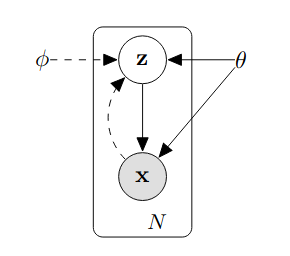
\includegraphics[width=4cm]{figures/vae_gm.png}
	\caption{Directed graphical model under consideration for VAE}
	\label{fig:boat1}
\end{figure}




\begin{figure}[htpb]
	\centering
	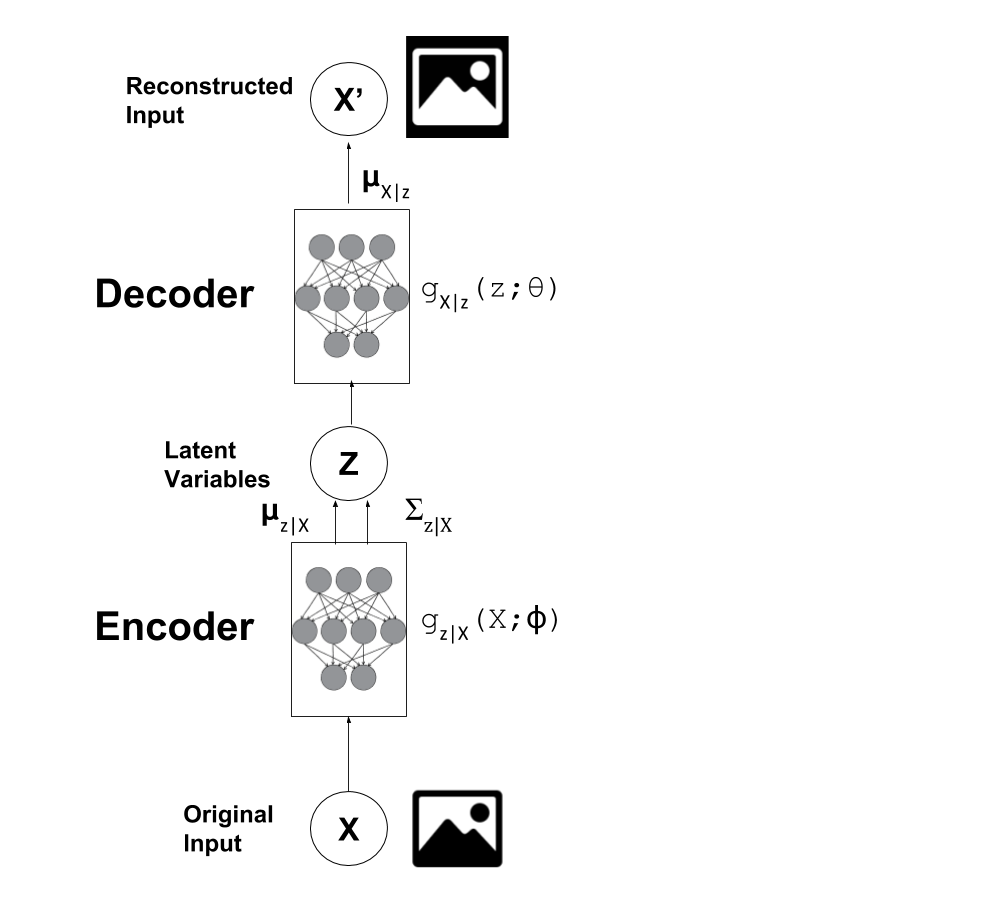
\includegraphics[width=10cm]{figures/vanilla_vae.png}
	\caption{Vanilla Variational Autoencoder}
	\label{fig:boat1}
\end{figure}






\part{Machine Learning}
\chapter{Probability Distribution}
\textbf{Definition}: \emph{conjugate priors} ---leads to posterior distributions having the same functional form as the prior.
\section{Binary Variables}
\subsection{Bernoulli distribution}
Considered a single binary random variable $x \in \{0, 1\}$. For example, flipping a coin, with $x = 1$ representing "heads", and $x = 0$ representing "tails". The probability distribution over $x$ can therefore be written in the form 
\begin{equation}
\mathrm{Bern}(x|\mu) = \mu^{x}(1-\mu)^{1-x}
\end{equation}
\begin{itemize}
	\item $\mathbb{E}[x]=\mu$
	\item $\mathrm{var}[x]=\mu(1-\mu)$
\end{itemize}
\subsection{Binomial distribution}
We can also work out the distribution of the number $m$ of observations of $x = 1$, given that the data set has size $N$. This is called the \emph{binomial distribution}
\begin{equation}
\mathrm{Bin}{(m|N,\mu)}=\binom{N}{m} \mu^m(1-\mu)^{N-m}
\end{equation}
\begin{itemize}
	\item $\mathbb{E}[m]=N\mu$
	\item $\mathrm{var}[m]=N\mu(1-\mu)$
\end{itemize}


\subsection{Beta distribution}
The \textbf{beta distribution} is introduced as a prior distribution $p(\mu)$ over the parameter $\mu$ for \textbf{binominal distribution} which keeps the \emph{conjugacy} property.

\begin{equation}
\mathrm{Beta}(\mu|a,b)=\frac{\Gamma{(a+b)}}{\Gamma{(a)}\Gamma{(b)}}\mu^{a-1}(1-\mu)^{b-1}
\end{equation}
\begin{itemize}
	\item $\mathbb{E}[\mu]=\frac{a}{a+b}$
\item $\mathrm{var}[\mu]=\frac{ab}{(a+b)^2(a+b+1)}$
\end{itemize}
The posterior distribution of $\mu$ is now obtained by multiplying the beta prior by the binomial likelihood function and normalizing, which has the form $p(\mu|m,l,a,b) \propto \mu^{m+a-1}(1-\mu)^{l+b-1}$
\begin{figure}[htpb]
	\centering
	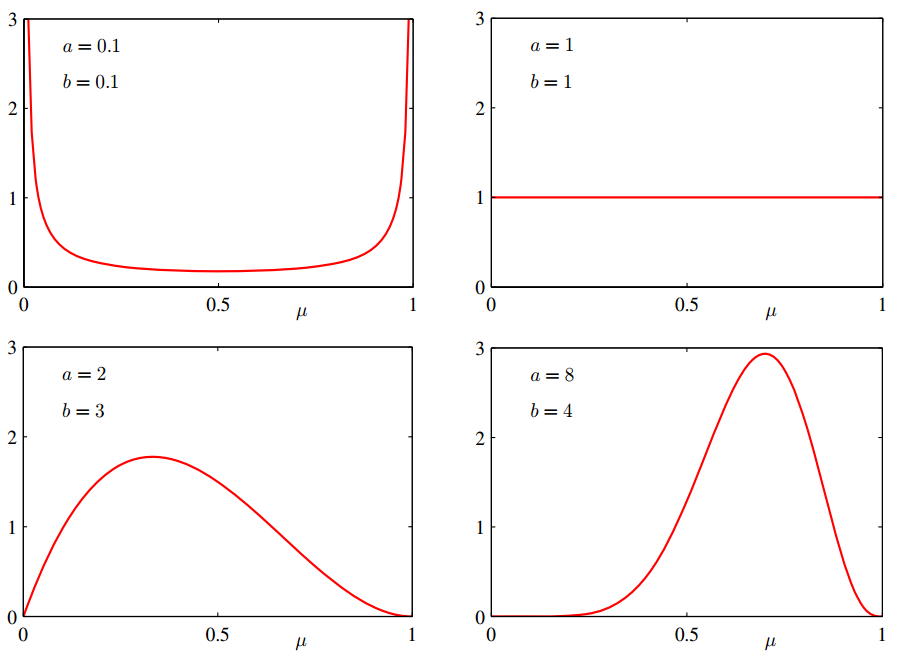
\includegraphics[width=10cm]{figures/beta_distribution.png}
	\caption{Plots of the beta distribution $\mathrm{Beta}{(\mu|a, b)}$ as a function of $\mu$ for various values of the
hyperparameters $a$ and $b$.}
	\label{fig:boat1}
\end{figure}


\section{Multinomial Variables}
We encounter discrete variables that can take on one of $K$
possible mutually exclusive states, then we replace $x$ in \emph{Bernoulli distribution} as a vector $\boldsymbol{x}$, such as $x=(0,0,1,0)^\top$. The distribution of $x$ is given 
\begin{equation}
p(x|\mu)=\prod_{k=1}^{K}\mu_k^{x_k}
\end{equation} 
This distribution can be regarded as a generalization of the Bernoulli distribution to more than two outcomes.

\subsection{Multinomial distribution}
We consider the joint distribution of the quantity $m_1,...,m_K$, conditioned on the parameters $\mu$ and on the total number $N$ of observations. $m_i$ is the occurrence number of $x_i$.
\begin{equation}
\mathrm{Mult}{(m_1m_2...m_K|\boldsymbol{\mu},N)}=\binom{N}{m_1,m_2,...m_K}\prod_{k=1}^K{\mu_{k}^{m_k}}
\end{equation}

\subsection{Dirichlet}
We now introduce a family of prior distribution for the parameters $\{\mu_k\}$ of the multinomial distribution, \emph{Dirichlet} distribution:
\begin{equation}
\mathrm{Dir}{(\boldsymbol{\mu}|\boldsymbol{\alpha})}=\frac{\Gamma{(\alpha_0)}}{\Gamma{(\alpha_1)}...\Gamma{(\alpha_K)}}\prod_{k=1}^{K}{\mu_{k}^{\alpha_k-1}}
\end{equation}
where $\alpha_0=\sum_{k=1}^{K}\alpha_k$
\begin{figure}[htpb]
	\centering
	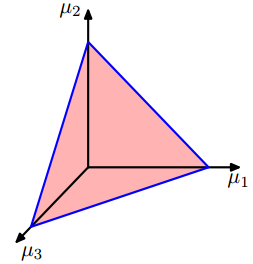
\includegraphics[width=4cm]{figures/dirichlet_simplex.png}
	\caption{The Dirichlet distribution over three variables $\mu_1, \mu_2, \mu_3$
		is confined to a simplex sof
the form shown, as a consequence of the constraints
$0\le \mu_k \le 1$ and $\sum_k{\mu_k} = 1$.}
	\label{fig:boat1}
\end{figure}
\begin{figure}[htpb]
	\centering
	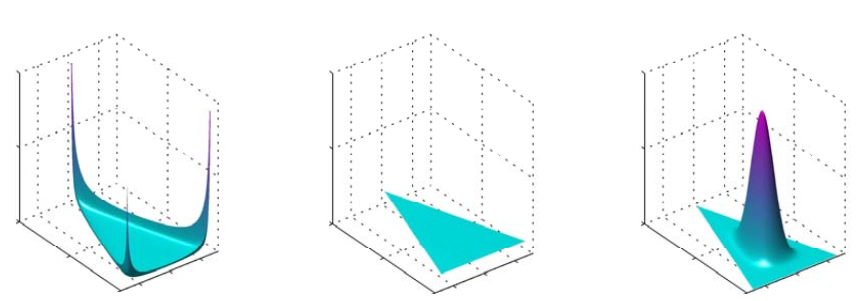
\includegraphics[width=\linewidth]{figures/dirichlet_dist.png}
	\caption{Plots of the Dirichlet distribution over three variables, where the two horizontal axes are coordinates
in the plane of the simplex and the vertical axis corresponds to the value of the density.}
	\label{fig:boat1}
\end{figure}


\chapter{Linear Models}
\section{Logistic Regression}
\subsection{Logistic sigmoid function}
$$f(x;w)=\sigma{(w^\top x)}=\frac{1}{1+e^{-w^\top x}}$$ 
\subsection{Loss function}
The \emph{Logistic Regression} model uses the interpretation of the function as a probability, $f(x;w)=p{(y=1|x,w)}$. Maximum likelihood fitting of this model minimizes the negative log-probability of the training labels, which could be written as:
$$NLL=-\sum_{n=1}^N{\log[\sigma{(w^\top x^{(n)})^{y^{(n)}}}(1-\sigma{(w^\top x^{(n)})})^{1-y^{(n)}}]}$$
or 
$$NLL=-\sum_{n:y^{(n)}=1}{\log{\sigma{(w^\top x^{(n)})}}}-\sum_{n:y^{(n)}=0}{\log{(1-\sigma{(w^\top x^{(n)})}})}$$ 
or using labels $z^{(n)} \in \{-1, +1\}$ where $z^{(n)}=(2y^{(n)}-1)$, and noticing $\sigma{(-a)}=1-\sigma{(a)}$:
$$NLL=-\sum_{n=1}^{N}{\log{\sigma{(z^{(n)}w^\top x^{(n)})}}}$$

\subsection{Gradient}
The derivative of the \emph{logistic sigmoid} as follows:
$$\frac{\partial{\sigma{(a)}}}{\partial{a}}=\sigma{(a)}(1-\sigma{(a)})$$
We use $\sigma_{n}=\sigma{(z^{(n)}w^\top x^{(n)})}$, then
\begin{equation}
\begin{split}\nabla_w{NLL} & =-\sum_{n=1}^{N}{\nabla_w{\log{(\sigma_{n})}}}=-\sum_{n=1}^{N}{\frac{1}{\sigma_{n}}\nabla_w{\sigma_{n}}}\\
&=-\sum_{n=1}^{N}{\frac{1}{\sigma_{n}}\sigma_{n}(1-\sigma_{n})\nabla_w{z^{(n)}w^{\top}x^{(n)}}}\\
&=-\sum_{n=1}^{N}{(1-\sigma_n)z^{(n)}x^{(n)}}\end{split}
\end{equation} 



\chapter{Kernel Methods}
Many linear parametric models can be re-cast into an equivalent ‘dual representation’ in which the predictions are also based on linear combinations of a kernel
function evaluated at the training data points. As we shall see, for models which are
based on a fixed nonlinear feature space mapping $\phi{(x)}$, the kernel function is given
by the relation
$$k(x,x^{\prime})=\phi{(x)}^{\top}\phi{(x)}$$
Many of them are \emph{stationary} kernels which have the property that $k(x,x^{\prime})=k(x-x^{\prime})$. (e.g. \emph{radial basis functions})
\section{Dual Representations}



\chapter{Dimensionality Reduction}
\section{Linear Discriminant Analysis}
\textbf{Linear Discriminant Analysis} or \textbf{LDA} is most commonly used as dimensionality reduction technique. The intuition behind LDA is that we would like to \emph{select the one of all possible lines that maximizes the separability of the scalars}.

\begin{figure}[htpb]
	\centering
	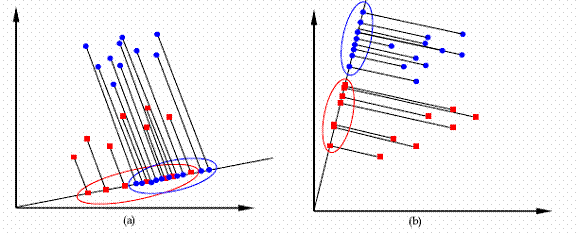
\includegraphics[width=\linewidth]{figures/lda.png}
	\caption{An illustration on the intuition behind LDA.}
	\label{fig:boat1}
\end{figure}

In order to find a good projection, we need to define a measure of separation between projections. The solution is to maximize a function that represents \textbf{the difference between the means, normalized by a measure of the within-class variability}.

Given a dataset $D=\{(x_i,y_i)\}_{i=1}^m,y_i \in \{0,1\}$ and $X_i, \mu_i, \Sigma_i$ denotes the \textbf{dataset}, \textbf{mean vector} and \textbf{covariance matrix} with label $i \in \{0,1\}$, then we define the $J$ is the objective function to be maximized: 
\begin{equation}
	\begin{split}
	J&=\frac{\left\lVert w^\top \mu_0-w^\top \mu_1 \right\lVert_2^2}{w^\top \Sigma_0w + w^\top \Sigma_1w} \\
	 &=\frac{w^\top (\mu_0-\mu_1)(\mu_0-\mu_1)^\top w}{w^\top (\Sigma_0 + \Sigma_1) w}
	\end{split}
\end{equation}

In order to find the optimum projection $w^*$, we need to express $J(w)$ as an explicit function of $w$, where $S_w$ is called \emph{within-class scatter matrix} and $S_b$ is called \emph{between-class scatter matrix}:
$$S_w=\Sigma_0 + \Sigma_1=\sum_{x\in X_0}{(x-\mu_0)(x-\mu_0)^\top}+\sum_{x\in X_1}{(x-\mu_1)(x-\mu_1)^\top}$$
$$S_b=(\mu_0-\mu_1)(\mu_0-\mu_1)^\top$$
To find the maximum of $J(w)$, we notice that the optimum solution $w^*$ is irrelevant to its magnitude, thus we assume $w^\top S_ww=1$, then
\begin{equation*}
\begin{aligned}
& \underset{w}{\mathrm{min}}
& & w^\top S_bw \\
& \mathrm{s.t.}
& & w^\top S_ww=1
\end{aligned}
\end{equation*}
With Lagrangian multiplier, we get 
$S_bw=\lambda S_ww$, notice that the direction of $S_bw$ is always the same as $\mu_0-\mu_1$, we assume $S_bw=\lambda{(\mu_0-\mu_1)}$. As a result, we get 
\begin{equation}
w=S_w^{-1}(\mu_0-\mu_1)
\end{equation}

\section{Principal Components Analysis}
\subsection{Singular Value Decomposition}
In linear algebra, the \textbf{singular-value decomposition} (\textbf{SVD}) is the generalization of the eigendecomposition of a \textbf{positive semidefinite normal matrix} (for example, a symmetric matrix with positive eigenvalues).

Formally, the singular-value decomposition of an $m\times n$ matrix $\mathbf{M}$ is a factorization of the form
\begin{equation}
	\mathbf{M} = \mathbf{U}\mathbf{S}\mathbf{V^\top}
\end{equation}
where 
\begin{itemize}
	\item $\mathbf{M}$: an $m\times m$ \textbf{unitary} matrix
	\item $\mathbf{S}$: an $ m\times n$ rectangular diagonal matrix with non-negative real numbers on the diagonal
	\item $\mathbf{V}$: an $n\times n$ \textbf{unitary} matrix
\end{itemize}

\subsection{Details}
\textbf{Principal Components Analysis} or \textbf{PCA} reduces the dimensionality of an $N\times D$ data matrix $\mathbf{X}$, by multiplying it by a $D \times K$ matrix $\mathbf{V}$. To keep the maths simpler, we will assume for the rest of this note that the $D$-dimensional feature vectors are \textbf{zero mean} (the average of the numbers in each column of $\mathbf{X}$ is zero). We centre the data to have this property before doing anything else.

We compute the covariance matrix of the points. As we're assuming $X$ is zero-mean, the covariance is $\Sigma=\frac{1}{N}X^\top X$. 
\begin{equation}
\begin{split}
\Sigma & =E(X^\top X) - \mu^\top \mu \\
& = E(X^\top X) \\
& \approx \frac{1}{N}X^\top X
\end{split}
\end{equation}

The covariance of  multivariate Gaussians can be used to describe an ellipsoidal ball that summarizes how the data is spread in space.\\ 

\begin{figure}[htpb]
	\centering
	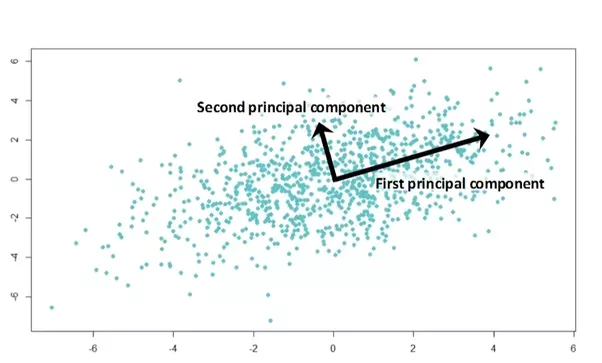
\includegraphics[width=8cm]{figures/pca.png}
	\caption{PCA example}
	\label{fig:boat1}
\end{figure}

Some axes of the ellipsoid are often very short, and the data is "squashed" into a ball that only significantly extends in some directions. The \textbf{eigenvectors} of the covariance matrix point along the axes of the ellipsoid, and the longest axes are the \textbf{eigenvectors} with \textbf{the largest eigenvalues}.

\subsection{PCA and SVD}
The truncated SVD view of PCA can find a low-dimensional vector representing either the rows or columns of a matrix. SVD finds both at once.

Singular Value Decomposition (SVD) factors a $N\times D$ matrix into a product of three matrices
$$\mathbf{X} \approx \mathbf{U}\mathbf{S}\mathbf{V}^{\top}$$
where
\begin{itemize}
\item $\mathbf{U}$ has size $N\times K$.
\item $\mathbf{S}$ is a diagonal $K \times K$ matrix.
\item $\mathbf{V}^\top$ has size $K \times D$.
\end{itemize}
The $\mathbf{V}$ matrix is the same as before, its columns (or the rows of $\mathbf{V}^\top$) contain eigenvectors of $\mathbf{X}^\top \mathbf{X}$. The columns of $\mathbf{U}$ contain eigenvectors of $\mathbf{X}\mathbf{X}^\top$. The rows of $\mathbf{U}$ give a $K$-dimensional embedding of the rows of $\mathbf{X}$. The columns of $\mathbf{V}^\top$ (or the rows of V) give a $K$-dimensional embedding of the columns of $\mathbf{X}$. 

A truncated SVD is known to be the best low-rank approximation of a matrix (as measured by square error). PCA is the linear dimensionality reduction method that minimizes the least squares error in the distortion if we project back to the original space: $\mathbf{X}\approx \mathbf{X}\mathbf{V}\mathbf{V}^\top$

\subsection{Further Details}
PCA is sensitive to the scaling of the variables. This means that whenever the different variables have different units (like temperature and mass), PCA is a somewhat arbitrary method of analysis. One way of making the PCA less arbitrary is to use variables scaled so as to have \textbf{unit variance}, by \textbf{standardizing the data} and hence use the autocorrelation matrix instead of the autocovariance matrix.

\textbf{Mean subtraction} is \textbf{necessary} for performing classical PCA to ensure that the first principal component describes the direction of maximum variance. If mean subtraction is not performed, the first principal component might instead correspond more or less to the mean of the data. A mean of zero is needed for finding a basis that minimizes the mean square error of the approximation.  

\subsection{PCA vs. LDA}
Both LDA and PCA are linear transformation techniques that are commonly used for dimensionality reduction. PCA can be described as an \textbf{"unsupervised"} algorithm while LDA is \textbf{"supervised"}.

\subsection{PCA Whitening}
The goal of whitening is to make the input less redundant, that is, the learning algorithms sees a training input where 1) the features are \textbf{less correlated} with each other, and 2) the features all have \textbf{the same variance}.

\subsubsection{Rotating the data}
As we mentioned in SVD that the matrix $\mathbf{V}$ is an unitary matrix, $x_{\mathrm{rot}}^{(i)}=x^{(i)}\mathbf{V}$ rotates the original data into orthogonal basis, which satisfies the first requirement --- the features are \emph{uncorrelated} (linear uncorrelated). 

\subsubsection{Unit variance}
To make each of our input features have unit variance, we can simply re-scale each feature $x_{\mathrm{rot},i}$ by multiplying $\frac{1}{\sqrt{\lambda_i}}$ where $\lambda_i$ is its corresponding eigenvalue (calculated in matrix $\mathbf{S}$):
\begin{equation}
x_{\mathrm{PCAwhite}}=\frac{x_{\mathrm{rot},i}}{\sqrt{\lambda_i}}
\end{equation}
 
This data now has covariance equal to identity matrix $\mathbf{I}$, the difference components of $x_{\mathrm{PCAwhite}}$ are \textbf{uncorrelated} and have \textbf{unit variance}.

\subsection{ZCA Whitening}
Finally, it turns out that this way of getting the data to have covariance identity $\mathbf{I}$ isn't unique. Concretely, if $\mathbf{R}^\top$ is any orthogonal matrix, so that it satisfies $\mathbf{R}\mathbf{R}^\top=\mathbf{R}^\top\mathbf{R}=\mathbf{I}$, then $x_{PCAwhite}\mathbf{R}^\top$ will also have identity covariance. In \textbf{ZCA whitening}, we choose $\mathbf{R}=\mathbf{V}$:
\begin{equation}
x_{\mathrm{ZCAwhite}}=x_{\mathrm{PCAwhite}}V^\top
\end{equation}

One defining property of ZCA transformation is that it results in whitened data that is \textbf{as close as possible} to the original data (in the least squares sense). In other words, if you want to minimize $\left\lVert \mathbf{X}-\mathbf{X}A^\top \right\rVert^2$ subject to $XA^\top$ being whitened, then you should take $A=W_{ZCA}$. Figure \ref{fig:zca_pca} is a 2D illustration:

\begin{figure}[htpb]
	\centering
	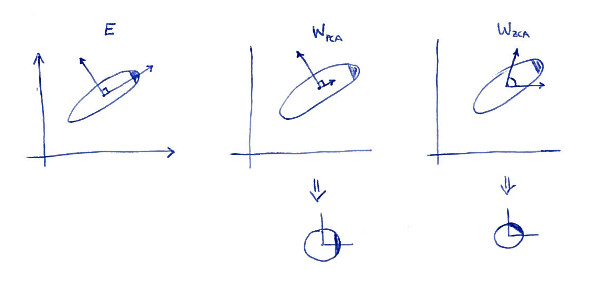
\includegraphics[width=\linewidth]{figures/zca.jpg}
	\caption{The difference of PCA and ZCA Whitening}
	\label{fig:zca_pca}
\end{figure}


\chapter{Independent Component Analysis}
\textbf{Independent Component Analysis} or \textbf{ICA}, similar to PCA, this will find a new basis in which to represent the data, but with a very different goal.

\section{Cocktail Party Problems}
Here, $n$ speakers are speaking simultaneously at a party, and any microphone placed in the room records only an overlapping combination of the $n$ speakers' voices. But let's say we have $n$ different microphones placed in the room, and because each microphone is a different distance from each of the speakers, it records a different combination of the speakers' voices. How can we separate out the original $n$ speakers' voices.


\chapter{Graphical Models}

\textbf{Probabilistic graphical models} offers several useful properties:
\begin{enumerate}
	\item They provide a simple way to visualize the structure of a probabilistic model and can be used to design and motivate new models.
	\item Insights into the properties of the model, including conditional independence properties, can be obtained by inspection of the graph.
	\item Complex computations, required to perform inference and learning in sophisticated models, can be expressed in terms of graphical manipulations, in which underlying mathematical expressions are carried along implicitly.
\end{enumerate} 
In general, graphical models can be classified as two classes:
\begin{itemize}
	\item \textbf{Bayesian Network}: \emph{directed graphical models}, are useful for expressing casual relationships between random variables.
	\item \textbf{Markov Random Field}: \emph{undirected graphical models} are better suited to expressing soft constraints between random variables.
\end{itemize}
For the purpose of solving inference problems, it is often convenient to convert \textbf{both} into different representation called \textbf{factor graph}.

\section{Bayesian Networks}
By considering the joint distribution over $K$ variables given by $p(x_1,...,x_K)$. By repeated application of the product rule of probability:
\begin{equation}
p(x_1,...,x_K)=p(x_K|x_1,...,x_{K-1})...p(x_2|x_1)p(x_1)
\end{equation}
The \emph{fully connected graph} can represent any form of probability distribution. It is the absence of links in the graph that conveys interesting information about the properties of the class of distributions the graph represents.

\subsection{Definition}
The joint distribution
defined by a graph is given by the product, over all of the nodes of the graph, of
a conditional distribution for each node conditioned on the variables corresponding
to the parents of that node in the graph. Thus, for a graph with $K$ nodes, the joint
distribution is given by 
\begin{equation}
p(\mathbf{x})=\prod_{k=1}^{K}{p(x_k|pa_k)}
\end{equation}
where $pa_k$ denotes the set of parents of $x_k$, and $\mathbf{x}=\{x_1,...,x_K\}$.

\subsection{Discrete Variables}
Exponential family probability distributions have particular nice properties if we choose the relationship between each parent-child pair in a directed graph to be \emph{conjugate}. When the parent and child node each correspond to discrete variables and when they each correspond to Gaussian variables, the relationship can be extended hierarchically to construct arbitrarily complex directed acyclic graphs.

\subsubsection{Logistic regression}
A logistic sigmoid function acting on a linear combination of the parent variables, giving 
$$p(y=1|x_1,...,x_M)=\sigma{(w_0+\sum_{i=1}^{M}{w_ix_i})}=\sigma{(\mathbf{w}^{\top}\mathbf{x})}$$
where $\mathbf{x}=(x_0,x_1,...,x_M)^{\top}$ is an (M+1)-dimensional vector of parent states.
\subsubsection{Linear-Gaussian models}
Consider an arbitrary directed acyclic graph over $D$ variables in which node $i$
represents a single continuous random variable $x_i$ having a Gaussian distribution.
The mean of this distribution is taken to be a linear combination of the states of its
parent nodes $pa_i$ of node $i$
$$p(x_i|pa_i)=\mathcal{N}{(x_i|\sum_{j\in pa_i}{w_{ij}x_j+b_i, v_i})}$$
where $w_{ij}$ and $b_i$ are parameters governing the mean, and $v_i$ is the variance of the
conditional distribution for $x_i$. The log of the joint distribution is then the log of the
product of these conditionals over all nodes in the graph and hence takes the form
$$\ln p{(\mathbf{x})}=\sum_{i=1}^{D}{\ln p(x_i|pa_i)}=-\sum_{i=1}^{D}{\frac{1}{2v_i}(x_i-\sum_{j \in pa_i}{w_{ij}x_j-b_j})^2 + \mathrm{const}}$$
where $\mathbf{x} = (x_1,..., x_D)^\top$ and 'const' denotes terms independent of $x$. We see that
this is a quadratic function of the components of $x$, and hence the joint distribution $p(x)$ is a multivariate Gaussian. 

\section{Conditional Independence}
Consider three variables $a$, $b$ and $c$, and we say $a$ and $b$ are \textbf{conditional independent} if 
\begin{equation}
p(a|b,c)=p(a|c)
\end{equation}
or 
\begin{equation}
\begin{split}
p(a,b|c) &=p(a|b,c)p(b|c) \\
&=p(a|c)p(b|c)
\end{split}
\end{equation}
or 
\begin{equation}
a \CI b \mid c
\end{equation}
Conditional independence properties play an important role in using probabilistic models for pattern recognition by simplifying both \textbf{the structure of a model} and \textbf{the computations needed to perform inference and learning under that model.}  \\

An important and elegant feature of graphical models is that conditional independence properties of the joint distribution can be \emph{read directly from the graph without having to perform any analytical manipulations.} The general framework for achieving this is called \emph{d-separation}.

\subsection{Three Example Graphs}
\subsubsection{Example 1}
\begin{figure}[htpb]
	\centering
	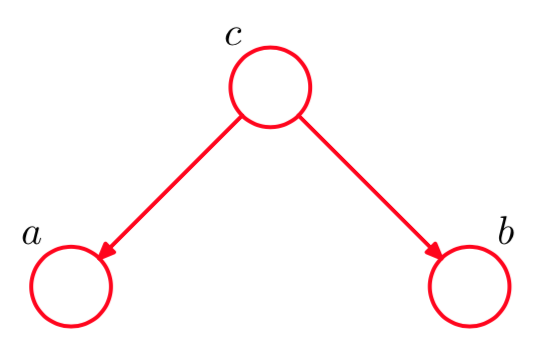
\includegraphics[width=6cm]{figures/bn_ex1_1.png}
	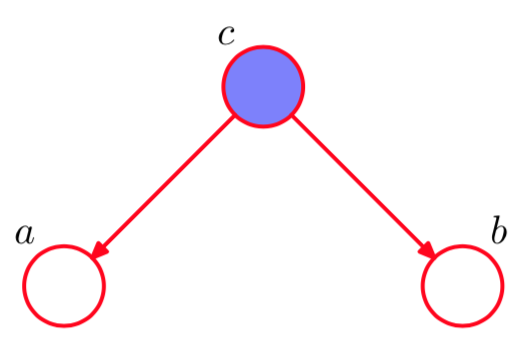
\includegraphics[width=6cm]{figures/bn_ex1_2.png}
	\caption{"tail-to-tail" structure}
	\label{fig:ci_example1}
\end{figure}
\begin{itemize}
	\item \textbf{none of the variables are observed}: $  a \nCI b \mid \emptyset$
	\item \textbf{conditioned on the variable c}: 
	\begin{equation}
	\begin{split}
		p(a,b|c) & = \frac{p(a,b,c)}{p(c)} \\
					& = \frac{p(a)p(c|a)p(b|c)}{p(c)} \\
					& =p(a|c)p(b|c)\\
	\end{split}
	\end{equation}
$$\Rightarrow a \CI b \mid c$$
\end{itemize}

\subsubsection{Example 2}
\begin{figure}[htpb]
	\centering
	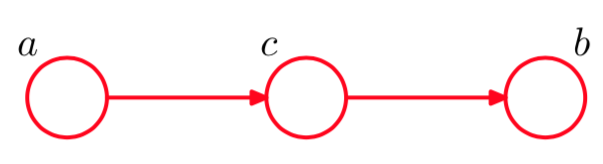
\includegraphics[width=6cm]{figures/bn_ex2_1.png}
	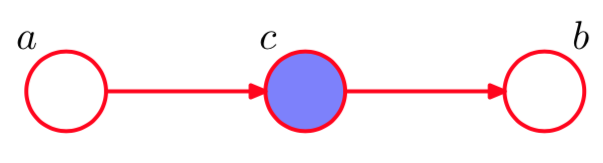
\includegraphics[width=6cm]{figures/bn_ex2_2.png}
	\caption{"head-to-tail" structure}
	\label{fig:ci_example2}
\end{figure}
\begin{itemize}
	\item \textbf{none of the variables are observed}: 
	$a \nCI b \mid \emptyset$
	\item \textbf{conditioned on the variable c}: 
	\begin{equation}
		\begin{split}
		p(a,b|c) & = \frac{p(a,b,c)}{p(c)} \\
		& = \frac{p(a)p(c|a)p(b|c)}{p(c)} \\
		& =p(a|c)p(b|c)\\
		\end{split}
	\end{equation}
	$$\Rightarrow a \CI b \mid c$$
\end{itemize}
\subsubsection{Example 3}
\begin{figure}[htpb]
	\centering
	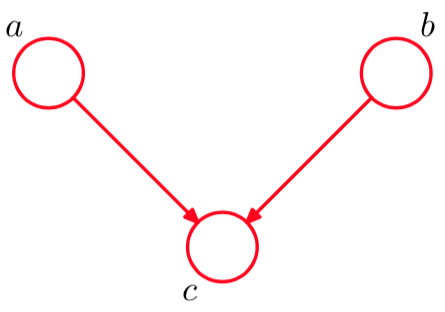
\includegraphics[width=6cm]{figures/bn_ex3_1.png}
	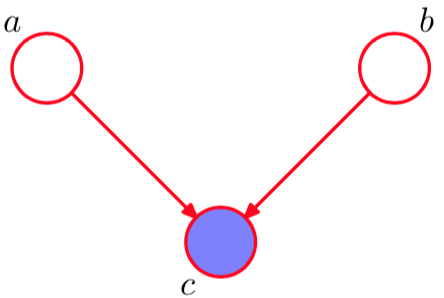
\includegraphics[width=6cm]{figures/bn_ex3_2.png}
	\caption{"tail-to-tail" structure}
	\label{fig:ci_example3}
\end{figure}
\begin{itemize}
	\item \textbf{none of the variables are observed}:
	\begin{equation}
		\begin{split}
		p(a,b,c) & = p(a)p(b)p(c|a,b)\\
		\end{split}
	\end{equation}
	\text{Marginalizing both sides over} c we obtain
	$$p(a,b)=p(a)p(b)$$
	$$\Rightarrow a \CI b \mid \emptyset$$
	\item \textbf{conditioned on the variable c}:
	\begin{equation}
		\begin{split}
		p(a,b|c) & = \frac{p(a,b,c)}{p(c)} \\
		& = \frac{p(a)p(b)p(c|a,b)}{p(c)} \\
		\end{split}
	\end{equation}
	$$\Rightarrow a \nCI b \mid c$$
\end{itemize}
\subsection{D-separation}


\section{Markov Random Fields}
\subsection{Conditional Random Field}

\chapter{Boosting}
\section{XGBoost}
XGBoost stands for "Extreme Gradient Boosting", where the term "Gradient Boosting" originates from the paper \emph{Greedy Function Approximation: A Gradient Boosting Machine}. The XGBoost is a decision tree ensemble model, whose objective function can be written in a general way as 
$$obj=\sum_{i=1}^{n}{l(y_i,\hat{y}_{t}^{(t)})+\sum_{i=1}^{t}{\Omega{(f_i)}}}$$

\subsection{Additive Training}
In order to find the \textbf{parameters} of trees, we need to learn those functions $f_i$, each containing the structure of the tree and the leaf scores. It is intractable to learn all trees at once, we use an additive strategy: fix what we have learned, and add one new tree at a time. We write the prediction value at step $t$ as $\hat{y}_i^{(t)}$. Then we have 
\begin{equation}
\begin{split}\hat{y}_i^{(0)} &= 0\\
\hat{y}_i^{(1)} &= f_1(x_i) = \hat{y}_i^{(0)} + f_1(x_i)\\
\hat{y}_i^{(2)} &= f_1(x_i) + f_2(x_i)= \hat{y}_i^{(1)} + f_2(x_i)\\
&\dots\\
\hat{y}_i^{(t)} &= \sum_{k=1}^t f_k(x_i)= \hat{y}_i^{(t-1)} + f_t(x_i)\end{split}
\end{equation}
It remains to ask: which tree do we want at each step? A natural thing is to add the one that optimizes our objective.
\begin{equation}
\begin{split}\mathrm{obj}^{(t)} & = \sum_{i=1}^n l(y_i, \hat{y}_i^{(t)}) + \sum_{i=1}^t\Omega(f_i) \\
& = \sum_{i=1}^n l(y_i, \hat{y}_i^{(t-1)} + f_t(x_i)) + \Omega(f_t) + \mathrm{constant}\end{split}
\end{equation}
If we consider using mean squared error (MSE) as our loss function, the objective becomes
\begin{equation}
\begin{split}\mathrm{obj}^{(t)} & = \sum_{i=1}^n (y_i - (\hat{y}_i^{(t-1)} + f_t(x_i)))^2 + \sum_{i=1}^t\Omega(f_i) \\
& = \sum_{i=1}^n [2(\hat{y}_i^{(t-1)} - y_i)f_t(x_i) + f_t(x_i)^2] + \Omega(f_t) + \mathrm{constant}\end{split}
\end{equation}
The form of MSE is friendly, with a first order term (usually called the residual) and a quadratic term. For other losses of interest (for example, logistic loss), it is \textbf{not so easy to get such a nice form}. So in the general case, we take the \textbf{Taylor expansion of the loss function up to the second order}:
\begin{equation}
\mathrm{obj}^{(t)} = \sum_{i=1}^n [l(y_i, \hat{y}_i^{(t-1)}) + g_i f_t(x_i) + \frac{1}{2} h_i f_t^2(x_i)] + \Omega(f_t) + \mathrm{constant}
\end{equation}
where the $g_i$ and $h_i$ are defined as
\begin{equation}
\begin{split}g_i &= \partial_{\hat{y}_i^{(t-1)}} l(y_i, \hat{y}_i^{(t-1)})\\
h_i &= \partial_{\hat{y}_i^{(t-1)}}^2 l(y_i, \hat{y}_i^{(t-1)})\end{split}
\end{equation}
After we remove all the constants, the specific objective at step $t$ becomes
\begin{equation}
\sum_{i=1}^n [g_i f_t(x_i) + \frac{1}{2} h_i f_t^2(x_i)] + \Omega(f_t)
\end{equation}

\subsection{Model Complexity}
We first refine the definition of the tree $f(x)$ as 
$$f_t{(x)}=w_{q(x)}, w\in\mathbb{R}^{T}, q:\mathbb{R}^{d}\to\{1,2,...,T\}$$
Here $w$ is the vector of scores on leaves, $q$ is a function assigning each data point to the corresponding leaf, and $T$ is the number of leaves. In XGBoost, we define the regularization term $\Omega{(f)}$ as follows:
\begin{equation}
\Omega{(f)}=\gamma T+\frac{1}{2}\lambda\sum_{j=1}^{T}{w_j^2}
\end{equation}
\subsection{The Structure Score}
We can write the objective value with the t-th tree as:
\begin{equation}
\begin{split}\mathrm{obj}^{(t)} &\approx \sum_{i=1}^n [g_i w_{q(x_i)} + \frac{1}{2} h_i w_{q(x_i)}^2] + \gamma T + \frac{1}{2}\lambda \sum_{j=1}^T w_j^2\\
&= \sum^T_{j=1} [(\sum_{i\in I_j} g_i) w_j + \frac{1}{2} (\sum_{i\in I_j} h_i + \lambda) w_j^2 ] + \gamma T\end{split}
\end{equation}
where $I_j=\{i|q(x_i)=j\}$ is the set of indices of data points assigned to the $j$-th leaf. Notice that in the second line we have changed the index of the summation because all the data points on the same leaf get the same score. We could further compress the expression by defining $G_j = \sum_{i\in I_j} g_i$ and $H_j = \sum_{i\in I_j} h_i$:
\begin{equation}
\mathrm{obj}^{(t)} = \sum^T_{j=1} [G_jw_j + \frac{1}{2} (H_j+\lambda) w_j^2] +\gamma T
\end{equation}
In this equation, wj are independent with respect to each other, the form $G_jw_j+\frac{1}{2}(H_j+\lambda)w^2_j$ is quadratic and the best w$_j$ for a given structure $q(x)$ and the best objective reduction we can get is:
\begin{equation}
\begin{split}w_j^\ast &= -\frac{G_j}{H_j+\lambda}\\
\mathrm{obj}^\ast &= -\frac{1}{2} \sum_{j=1}^T \frac{G_j^2}{H_j+\lambda} + \gamma T\end{split}
\end{equation}
The last equation measures how good a tree structure $q(x)$ is.

\begin{figure}[htpb]
	\centering
	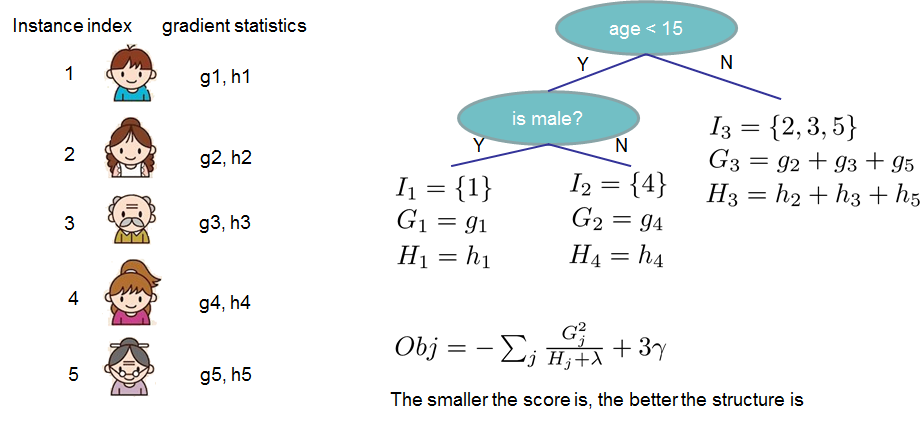
\includegraphics[width=13cm]{figures/xgboost_struct_score.png}
	\caption{Example of how objective of XGBoost is calculated.}
	\label{fig:boat1}
\end{figure}

\subsection{Learn The Tree Structure}
Now that we have a way to measure how good a tree is, ideally we would enumerate all possible trees and pick the best one. In practice this is intractable, so we will try to optimize one level of the tree at a time. Specifically we try to split a leaf into two leaves, and the score it gains is
\begin{equation}
Gain = \frac{1}{2} \left[\frac{G_L^2}{H_L+\lambda}+\frac{G_R^2}{H_R+\lambda}-\frac{(G_L+G_R)^2}{H_L+H_R+\lambda}\right] - \gamma
\end{equation}
This formula can be decomposed as 
\begin{enumerate}
	\item the score on the new left leaf
	\item the score on the new right leaf
	\item the score on the original leaf
	\item the regularization on the additional leaf
\end{enumerate}
We can see an important fact here: if the gain is smaller than $\gamma$, we would do better not to add that branch. This is exactly the \textbf{pruning} techniques in tree based models! By using the principles of supervised learning, we can naturally come up with the reason these techniques work :)

For real valued data, we usually want to search for an optimal split. To efficiently do so, we place all the instances in sorted order, like the following picture.
\begin{figure}[htpb]
	\centering
	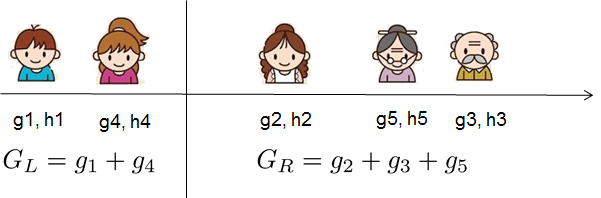
\includegraphics[width=10cm]{figures/split_find.png}
	\caption{How to find splits in XGBoost.}
	\label{fig:boat1}
\end{figure}
A left to right scan is sufficient to calculate the structure score of all possible split solutions, and we can find the best split efficiently.


\chapter{Sampling Methods}
\section{Standard Distributions}

\section{Importance Sampling}
One of the principal reasons for wishing to sample from complicated probability distributions is to be able to evaluate expectations of the form 
\begin{equation}
\mathbb{E}{(f)}=\int{f{(\mathbf{z})}p{(\mathbf{z})}}d{\mathbf{z}}
\end{equation}
One simple strategy for evaluating expectations would be to discretize $z$-space into a uniform grid and evaluate the integrand as a sum of the form
\begin{equation}
\mathbb{E}{(f)} \simeq \sum_{l=1}^{L}{p{(\mathbf{z}^{(l)})} f{(\mathbf{z}^{(l)})}}
\end{equation}
An obvious problem with this approach is that \textbf{the number of terms in the summation grows exponentially with the dimensionality of z}.

Importance sampling is based on the use of a proposal distribution $q(z)$ from which it is easy to draw samples. We can then express the expectation in the form of a finite sum over samples $\{\mathbf{z}^{(l)}\}$ drawn from $q(\mathbf{z})$

\begin{equation}
\begin{split}
\mathbb{E}{[f]} & = \int{f(\mathbf{z})p(\mathbf{z})d\mathbf{z}} \\
& = \int{f(\mathbf{z}) \frac{p(\mathbf{z})}{q(\mathbf{z})} p(\mathbf{z})d\mathbf{z}} \\
& \simeq \frac{1}{L} \sum_{l=1}^{L}{\frac{ p(\mathbf{z}^{(l)}) }{q(\mathbf{z}^{(l)})} } f(\mathbf{z}^{(l)})\\
\end{split}
\end{equation}

\part{Algorithm}
\chapter{Trie}
\textbf{Trie} is a kind of digital search tree. Trie is an efficient indexing model, which is indeed also a kind of \textbf{deterministic finite automaton} (DFA).
\begin{figure}[htpb]
	\centering
	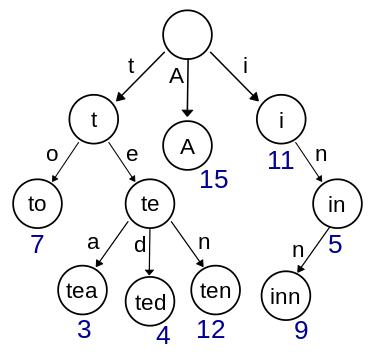
\includegraphics[width=8cm]{figures/trie.png}
	\caption{Trie}
	\label{fig:boat1}
\end{figure}
\section{Tripple-Array Trie}
\subsection{Structure}
The tripple-array structure is composed of:
\begin{itemize}
	\item \textbf{base}: Each element in base corresponds to a node of the trie. For a trie node s, $base[s]$ is the starting index within the next and check pool for the row of the node s in the transition table. 
	\item \textbf{next}: This array, in coordination with check, provides a pool for the allocation of the sparse vectors for the rows in the trie transition table. The vector data, that is, the vector of transitions from every node, would be stored in this array. 
	\item \textbf{check}: This array works in parallel to next. It marks the owner of every cell in next. This allows the cells next to one another to be allocated to different trie nodes. That means the sparse vectors of transitions from more than one node are allowed to be overlapped.
\end{itemize}
\textbf{Definition}: For a transition from state s to t which takes character c as the input, the condition maintained in the tripple-array trie is:\\
\begin{equation}
\begin{split}
& check[base[s]+c]=s \\
& next[base[s]+c]=s
\end{split}
\end{equation}
\begin{figure}[htpb]
	\centering
	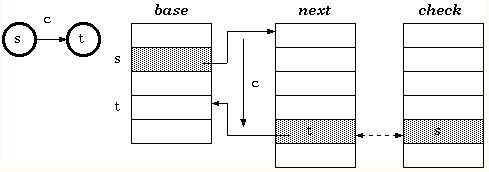
\includegraphics[width=12cm]{figures/tripple_array_trie.png}
	\caption{Tripple-array trie}
	\label{fig:boat1}
\end{figure}
\subsection{Walking}
\begin{algorithmic}
	\STATE $t\gets base[s] + c$
	\IF {$check[t] = s$} 
	\STATE $\mathrm{next state}\gets next[t]$
	\ELSE
	\STATE $\mathrm{fail}$
	\ENDIF 
\end{algorithmic}


\section{Double-Array Trie}
The tripple-array structure for implementing trie appears to be well defined, but is still not practical to keep in a single file. The \emph{next/check} pool may be able to keep in a single array of integer couples, but the base array does not grow in parallel to the pool, and is therefore usually split.

\subsection{Structure}
Instead of indirectly referencing through state numbers as in tripple-array trie, nodes in double-array trie are linked directly within the \textbf{base/check} pool.
\textbf{Definition}: For a transition from state $s$ to $t$ which takes character $c$ as the input, the condition maintained in the double-array trie is:\\
\begin{equation}
\begin{split}
& check[base[s]+c]=s \\
& base[s]+c=t
\end{split}
\end{equation}
\begin{figure}[htpb]
	\centering
	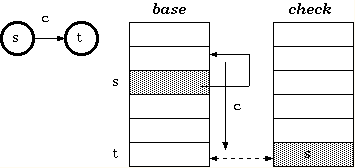
\includegraphics[width=9cm]{figures/double_array_trie.png}
	\caption{Double-array trie}
	\label{fig:boat1}
\end{figure}

\subsection{Walking}
\begin{algorithmic}
	\STATE $t\gets base[s] + c$
	\IF {$check[t] = s$} 
	\STATE $\mathrm{next state}\gets t$
	\ELSE
	\STATE $\mathrm{fail}$
	\ENDIF 
\end{algorithmic}


\section{An Efficient Language Model Using Double-Array Structure}

\part{Extreme Computing}
\chapter{Extreme Computing Algorithms}
\section{Bloom Filter}
\begin{figure}[htpb]
	\centering
	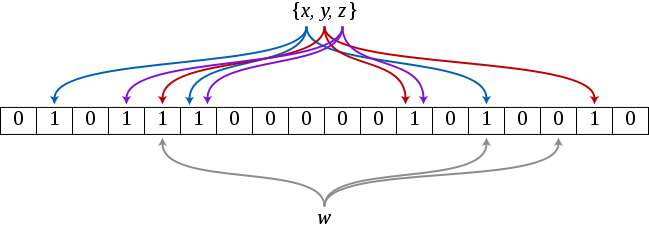
\includegraphics[width=10cm]{figures/bloom_filter.png}
	\caption{Bloom filter structure}
	\label{fig:boat1}
\end{figure}

The structure of a bloom filter can be explained here. Essentially, a bloom filter
is implemented by a bit array with N entries and a set of k hash functions, $h_1 , ..., h_k$. We assume the hash functions are independent and map a uniformly random selected
key to every entry with equal probability. Initially, all entries in the bit array are then
set to zero. Insertion and query operations define following actions:
\begin{itemize}
	\item \textbf{Insert key $x$}: with k hash functions, we compute $ h_1(x), ..., h_k(x)$ values and
	set the entries location in positions $h_1(x), ..., h_k(x)$ in the bit array with 1.
	\item \textbf{Query key $x$}: given the key w, we compute $h_1(w), ..., h_k(w)$, if all values of entries located in position $h_1(w),...,h_k(w)$ are 1 then the bloom filter returns
	true. Otherwise, false is returned.
\end{itemize}

The \textbf{false positive rate} in the bloom filter depends on $m$ (\textbf{the number of bits in array}), $k$ (\textbf{the number of hash functions}) and $n$ (\textbf{the number of inserted elements}).

the probability of a bit is not set to $1$ by a specific hash function in one insertion is
$$1-\frac{1}{m}$$
Note that hash functions are independent; thus, the probability of a bit not set to $1$ by $k$ hash functions is just
$$(1-\frac{1}{m})^k$$
After $n$ elements insertion, the probability becomes
$$(1-\frac{1}{m})^{kn}$$
Now we consider testing a key $w$ which is not in the set, then the probability
that the $k$ computed positions $h_1(w), ...h_k(w)$ by hash functions $h_1 , ...h_k$ are all $1$ is
$$(1-[1-\frac{1}{m}]^{kn})^k \approx (1-e^{-\frac{kn}{m}})^k$$
\section{Resevoir Sampling}
\textbf{Resovoir sampling} enables sampling from a large dataset with one iteration, which is broadly applied in search engines.

\subsection{Sample One Line}
\begin{lstlisting}

// Uniformly sample one line
import sys
import random

line_number = 0
for line in sys.stdin:
	if random.randint(0, line_number) == 0:
		resevoir = line.strip()
	line_number += 1
print(resevoir)
\end{lstlisting}

\subsection{Proof}
\begin{itemize}
	\item \textbf{Base}: One line with probability $1$.
	\item \textbf{Inductive}: Assume $n$ lines were sampled with probability $\frac{1}{n}$ each.
	When the $n + 1$th line is added, the resevoir is kept with probability $\frac{n}{n+1}$. Thus the first $n$ lines each have probability 
	$$\frac{1}{n} \times \frac{n}{n+1}=\frac{1}{n+1}$$
	And the $n+1$th line also has probability $\frac{1}{n+1}$ by construction.
\end{itemize}

\subsection{Sample Multiple Lines}
\begin{lstlisting}

// Uniformly sample multiple lines
import sys
import random

SAMPLES = 10
resevoir = []

# Fill resevoir
for i in range(SAMPLES):
	resevoir.append(sys.stdin.readline())
line_number = SAMPLES

# Substitute an entry with probability |samples|/|lines|
for line in sys.stdin:
	generated = random.randint(0, line_number)
	if generated < SAMPLES:
		resevoir[generated] = line
	line_number += 1
print("".join(resevoir), end="")
\end{lstlisting}

\chapter{Frequent Pattern Mining}
\large{\textbf{"- Which pages are getting an unusual hit in the last 30 minutes? \\
		   \indent- Which categories of items are now hot?}}\\


Frequent pattern mining refers to finding patterns that occur more frequently than a pre-specified threshold value. Frequent pattern mining over data streams differ from conventional one:
\begin{itemize}
	\item can not afford multiple passes 
	\begin{itemize}
		\item minimize requirements in terms of memory
		\item trade off between storage, complexity and accuracy
		\item only get one look
	\end{itemize}
	\item frequent items and itemsets are usually the final output
\end{itemize}

\section{Lossy Counting}
\textbf{Step 1}: Divide the incoming data stream into windows. 
\begin{figure}[htpb]
	\centering
	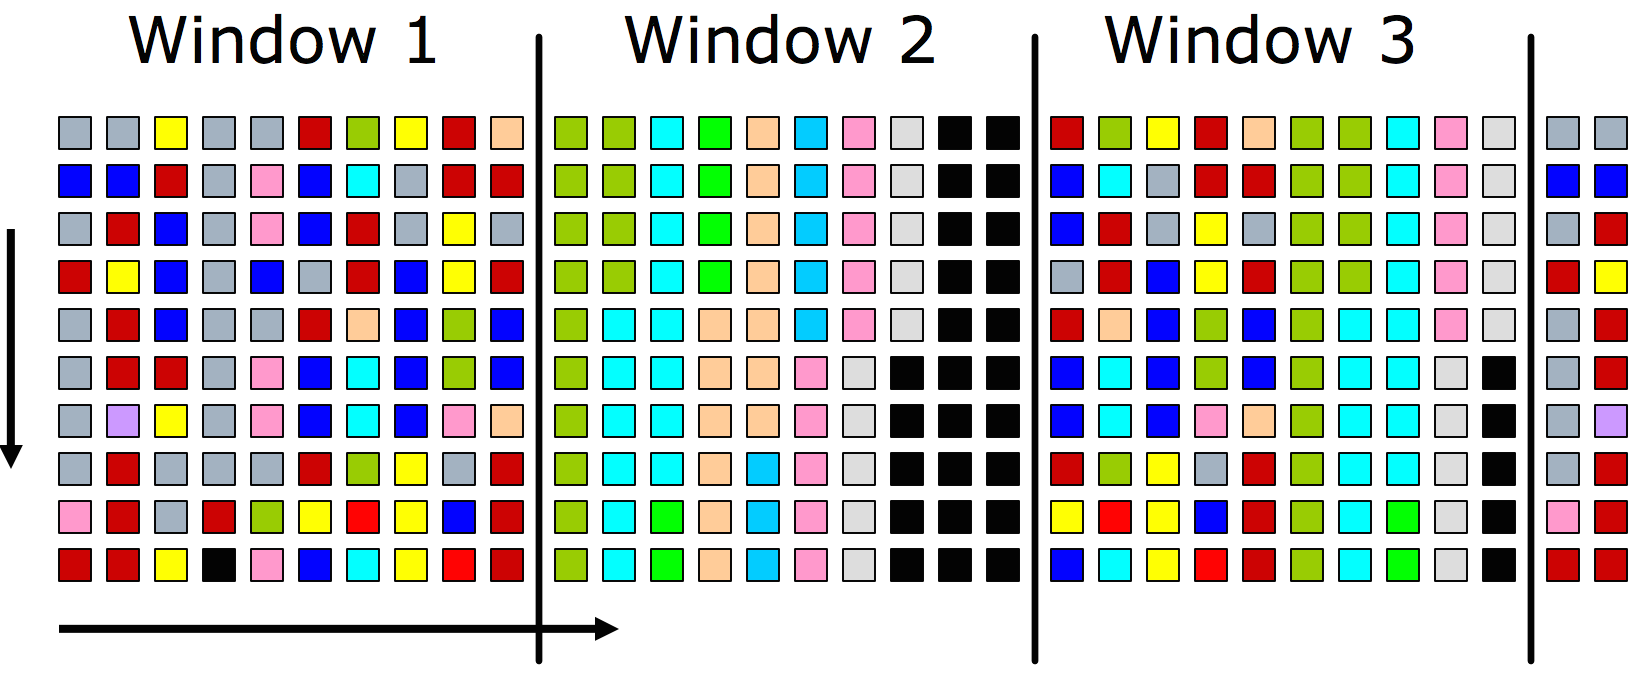
\includegraphics[width=9cm]{figures/step_1_lossy_counting.png}
	\caption{Split input stream into windows}
	\label{fig:boat1}
\end{figure}
\\\\
\textbf{Step 2}: Increment the frequency count of each item according to the new window values. After each window, decrement all counters by 1.
\begin{figure}[htpb]
	\centering
	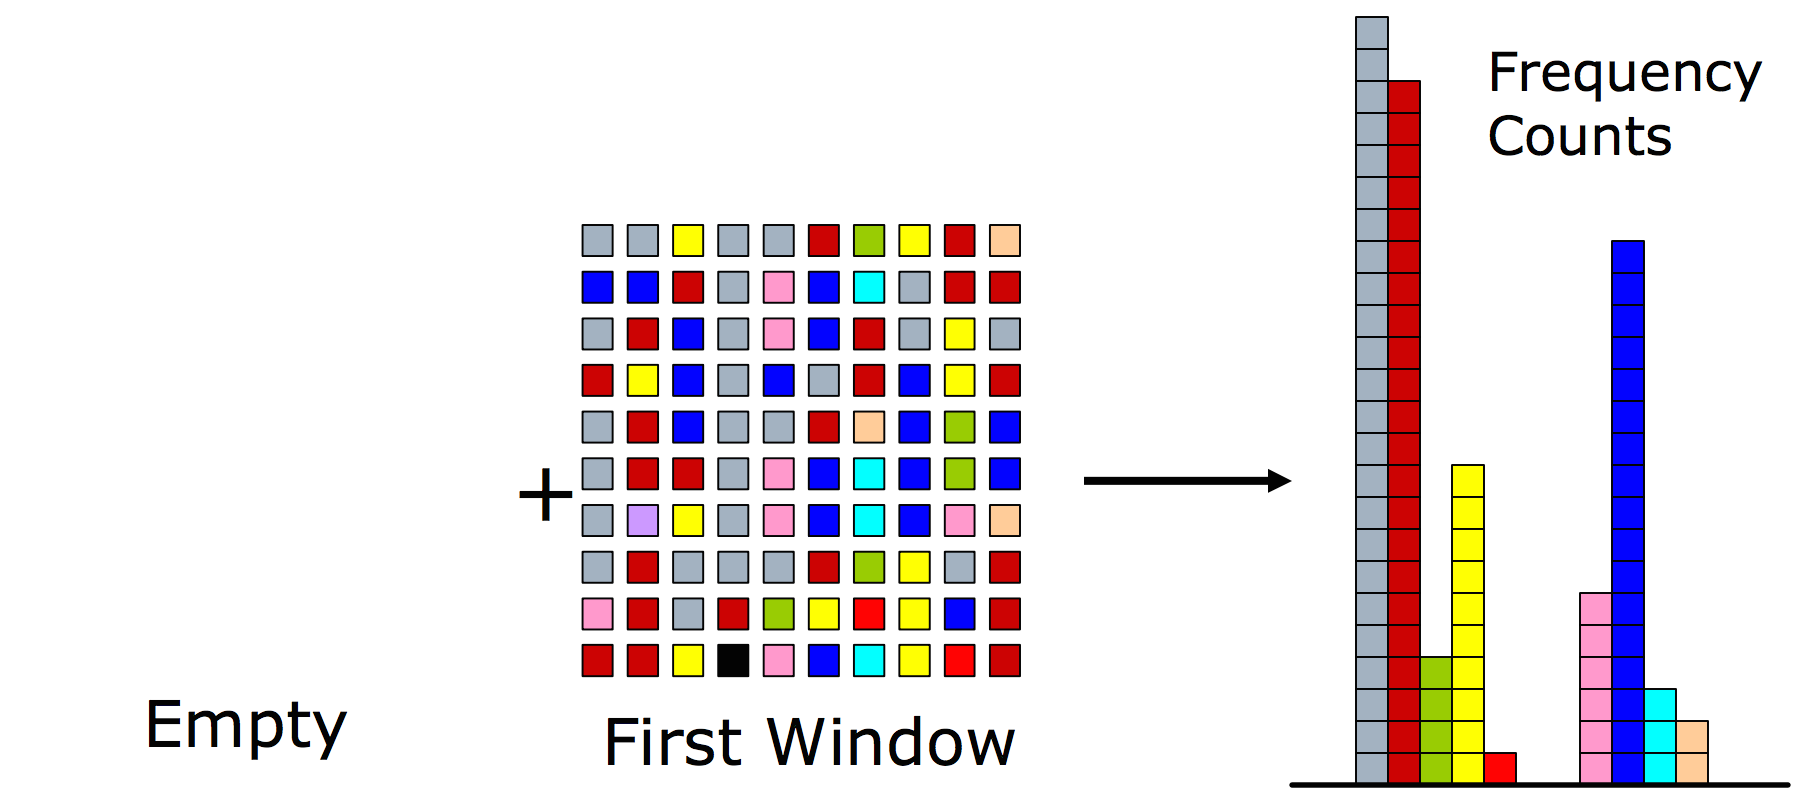
\includegraphics[width=10cm]{figures/step_2_lossy_counting.png}
	\caption{Increment frequency counts --- At window boundary adjust counts}
	\label{fig:boat1}
\end{figure}
\\\\
\textbf{Step 3}: Repeat --- Update counters and after each window, decrement all counters by 1.
\begin{figure}[htpb]
	\centering
	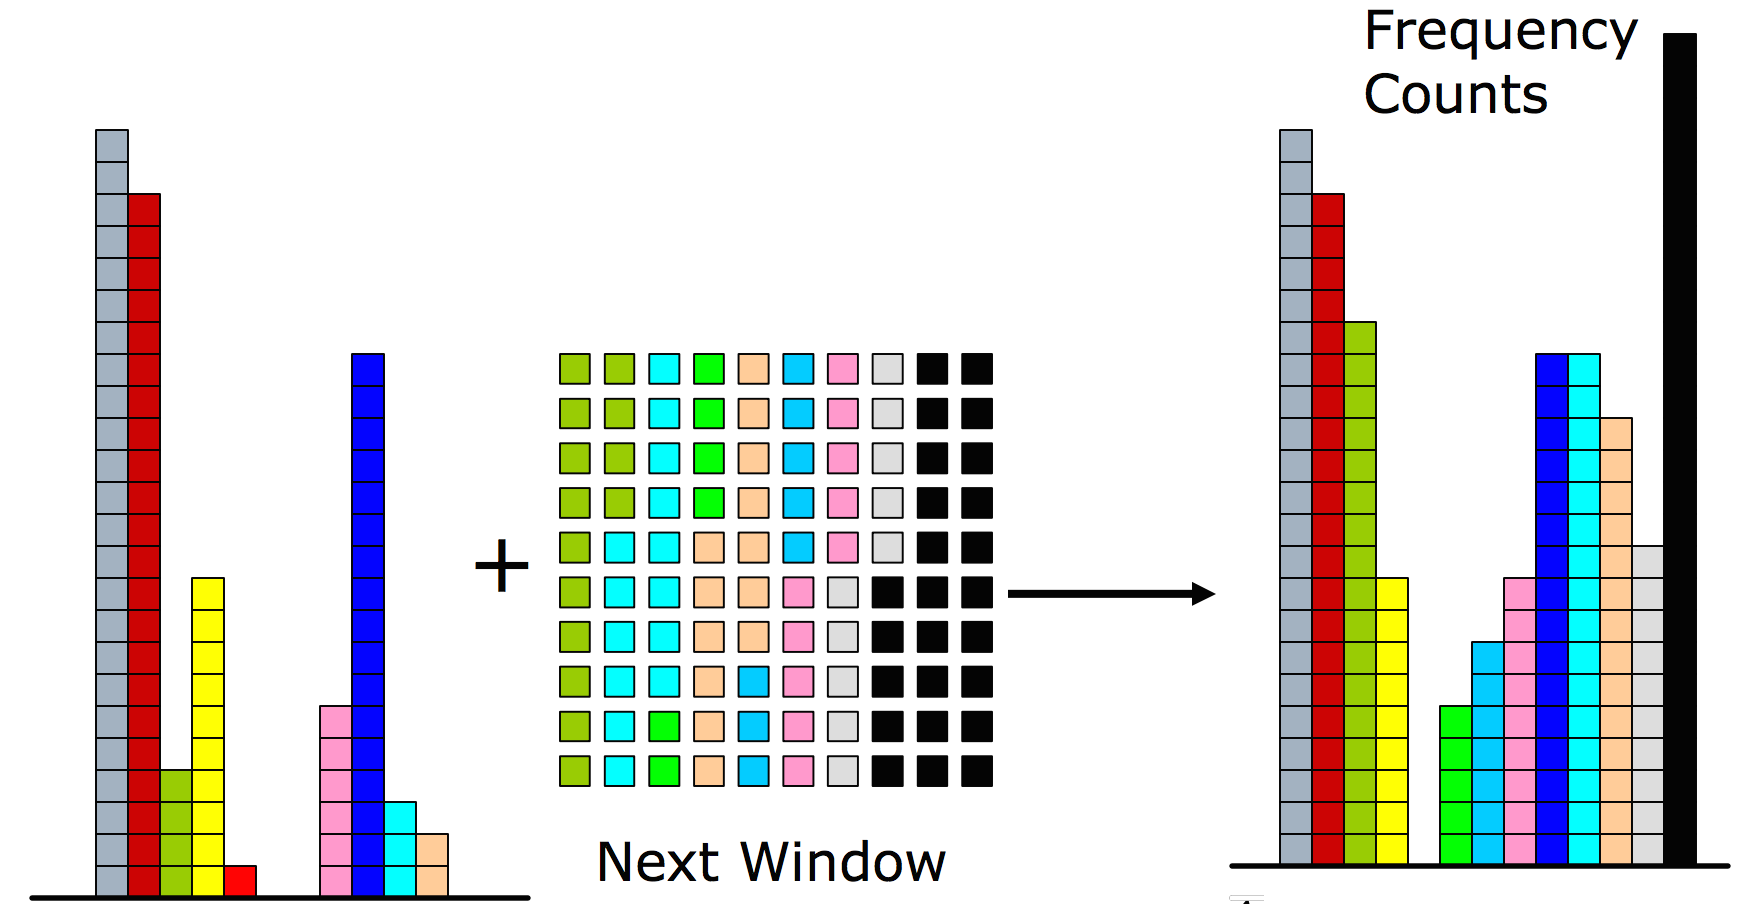
\includegraphics[width=9cm]{figures/step_3_lossy_counting.png}
	\caption{Update counters and at window boundary decrement all items by 1}
	\label{fig:boat1}
\end{figure}

\subsection{Implementation}
\begin{enumerate}
	\item user supplies two parameters support $s$ and error $\epsilon$
	\item simple data structure, maintaining triplets of data items $e$, their associated frequencies $f$, and the maximum possible error $\Delta$ in $f$: $(e, f, \Delta)$.
	\item The stream is conceptually divided into buckets of width $w=\frac{1}{\epsilon}$ --- Each bucket labeled by a value $\frac{N}{w}$ where $N$ starts from $1$ and increases by $1$.
	\item For each incoming item, the data structure is checked
	\begin{itemize}
		\item If an entry exists, increment frequency
		\item Otherwise, add new entry with $\Delta=b_{current}-1$ where $b_{current}$ is the current bucket label
	\end{itemize}  
	\item When switching to a new bucket, all entries with $f+\Delta < b_{current}$ are released.
\end{enumerate}

\subsection{Output}
The most frequently viewed items "survive". Given a frequency threshold $f$, a frequency error $\epsilon$, and total number of elements $N$, then frequency error $\le$ number of windows ($\epsilon N$). Thus, the output can be expressed as follows: Elements with count exceeding $fN - \epsilon N$. \\

Worst case we need $\frac{1}{\epsilon} * \log{(\epsilon N)}$ counters.\\

For example, we may want to print the Facebook pages of people who get hit more than 20\%, with an error threshold of 2\%. For frequency $f$ = 20\%, $\epsilon$ = 2\%, all elements with true frequency exceeding $f$ = 20\% will be output --- there are no false negatives. But we undercount. The output frequency of an element can be less than its true frequency by at most 2\%. False positives could appear with frequency between 18\% -- 20\%. Last, no element with frequency less than 18\% will be output.

Given window of size $\frac{1}{\epsilon}$, the following guarantees hold:
\begin{itemize}
	\item Frequencies are underestimated by at most $\epsilon * N$
	\item No false negatives
	\item False positives have true frequency of at least $f*N - \epsilon*N$
\end{itemize}

\section{Sticky Sampling}
This is another technique for counting but probabilistic. Here the space consumption is \textbf{independent} of the length of the stream $N$.
\begin{figure}[htpb]
	\centering
	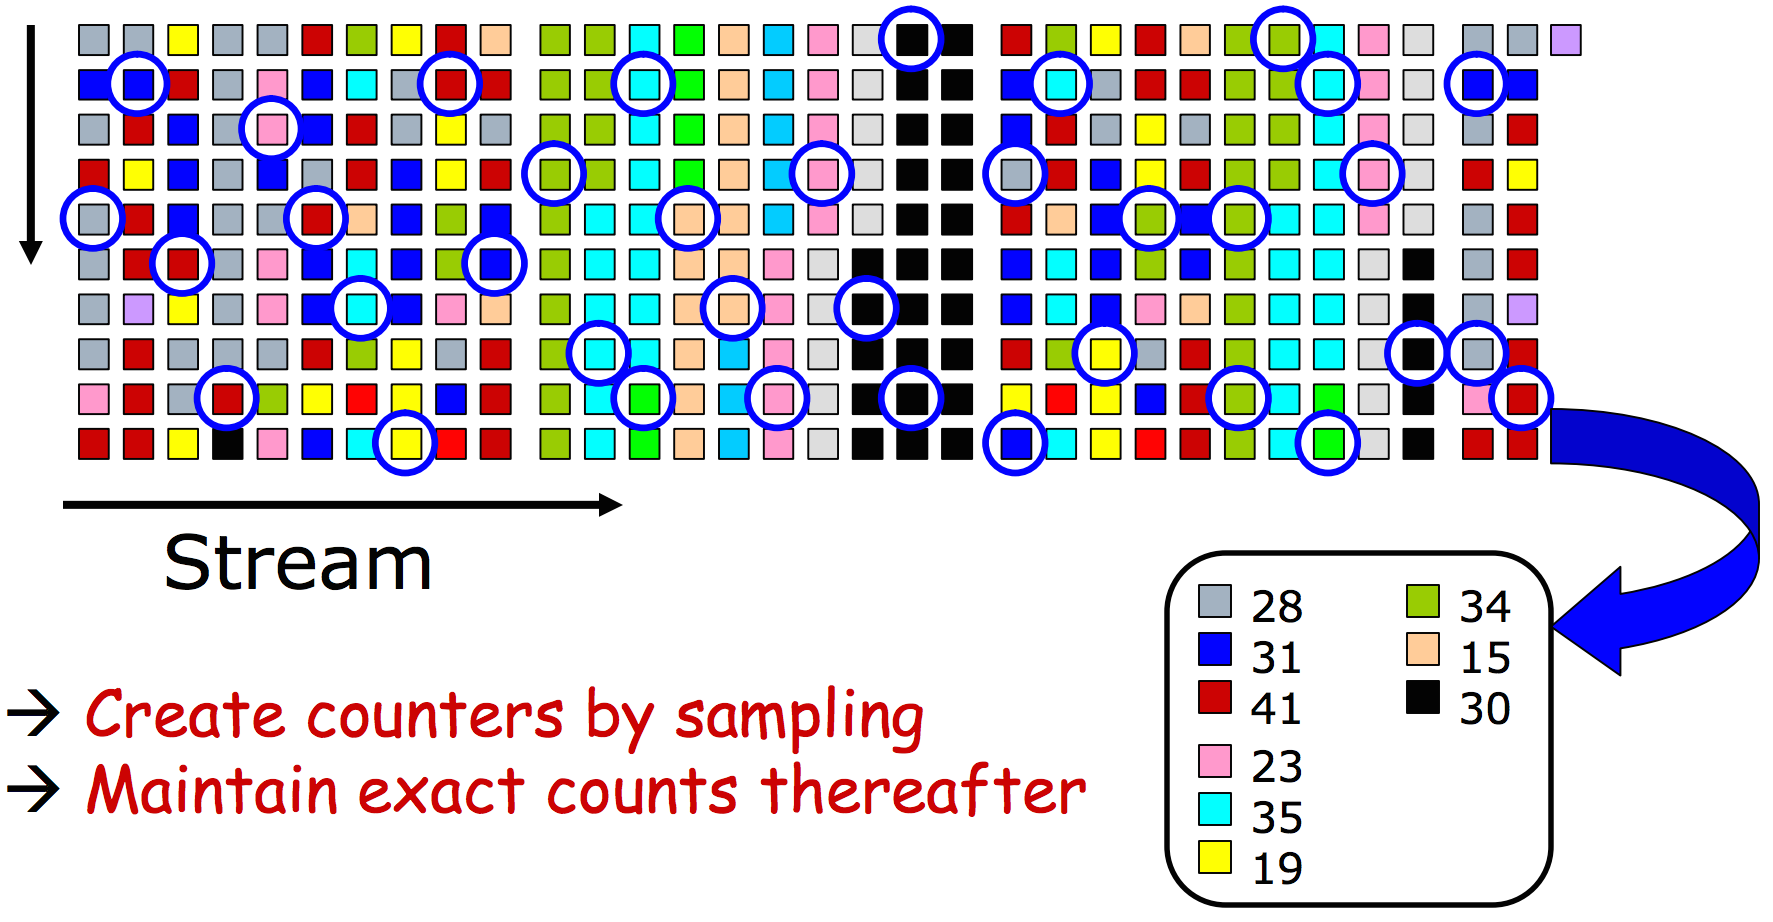
\includegraphics[width=11cm]{figures/step1_sticky_sampling.png}
	\caption{Sticky sampling}
	\label{fig:boat1}
\end{figure}

The user defines the frequency threshold $f$, the error $\epsilon$ but also the probability of failure $\delta$.

The logic is the following: For each incoming item, if an entry exists we increase its frequency. Otherwise we may select the item based on a probability $\frac{1}{r}$. This is called sampling. We gradually increase the sampling rate (starting at $r=1$) as more elements are processed. Upon a sampling rate change, we scan all existing entries. For each entry, we toss an unbiased coin and we decrease the item's frequency for each unsuccessful toss, until the coin toss becomes successful or the frequency becomes $0$ at which we release the entry.

The sampling rate is adjusted according to the following formula
$$t = \frac{1}{\epsilon} * \log{(\frac{1}{f*\delta})}$$
The first $t$ elements are sampled at rate $r=1$, the next $2t$ elements at rate $r=2$, the next $4t$ at rate $r=4$ etc.

\subsection{Output}
Same as lossy counting: Given a frequency threshold $f$, a frequency error $\epsilon$, and total number of elements $N$, the output can be expressed as follows: Elements with count exceeding $fN - \epsilon N$. \\

Number of counters expected (probabilistically): $\frac{2}{\epsilon}*\log{(\frac{1}{f*\delta})}$ \\

It's worth noting that the number of counters here is independent of N, the length of the stream. The same guarantees as lossy counting apply here:
\begin{itemize}
	\item Frequencies are underestimated by at most $\epsilon * N$
	\item No false negatives
	\item False positives have true frequency of at least $f*N - \epsilon*N$
\end{itemize}

\section{Comparison}
\begin{itemize}
	\item Lossy counting is more accurate but Sticky Sampling requires \textbf{constant space}. Lossy Counting space requirements \textbf{increase logarithmically} with the length of the stream $N$.
	\item Sticky sampling remembers every unique element that gets sampled, whereas Lossy Counting chops off low frequency elements quickly leaving only the high frequency ones.
	\item Sticky sampling can support infinite streams while keeping the same error guarantees as Lossy Counting.
\end{itemize}



\part{Front-end Web Development}
\chapter{HTML5}
\href{https://www.w3.org/TR/html5/introduction.html#a-quick-introduction-to-html}{\textbf{HTML5}} is the World Wide Web's core markup language. Originally, HTML was primarily designed as a language for semantically describing scientific documents.



\bibliographystyle{abbrvnat}

\bibliography{note}

%----------------------------------------------------------------------------------------

\end{document}